% vim: ft=tex
\documentclass[a4paper]{report}
\usepackage[english,ngerman]{babel}
\usepackage[utf8]{inputenc}
\usepackage[a4paper]{geometry}
\geometry{verbose, marginparwidth=15mm, marginparsep=3mm, tmargin=25mm}
\usepackage[svgnames, table]{xcolor}
\usepackage{graphicx}
\usepackage[hyphens]{url}
\usepackage[flushmargin,hang]{footmisc}
\usepackage{hyperref}
\usepackage{xspace} % space, but not before punctuation
\usepackage[hypcap]{caption} % link to top of tables and figures, not to bottom caption
\usepackage{microtype} % letter spacing

% paragraph spacing, no indentation, with normal list spacing
\usepackage[parfill]{parskip} % no idented first line of each paragraph
\usepackage{enumitem}
\newlength\docparskip
\parskip=10pt
\setlength{\docparskip}{\parskip}
\setlist{nosep, itemsep=5pt, parsep=0pt, before={\parskip=5pt}, after={}}

\usepackage{multirow}
\usepackage{longtable}
\usepackage{pgfgantt}

\usepackage{amssymb} % for \checkmark
\usepackage{textgreek} % for \textMu
\usepackage{enumitem} % for \begin{itemize}[label={...}]
\usepackage[export]{adjustbox} % left/right aligned images
\usepackage{newfloat}
\usepackage{tikz}
\usetikzlibrary{arrows,decorations.pathmorphing,backgrounds,fit,positioning,shapes.symbols,chains,shapes.geometric,shapes.arrows,calc}
\usepackage[
backend=biber,
hyperref=true,
url=true,
isbn=false,
backref=false,
% style=custom-numeric-comp,
citereset=chapter,
maxcitenames=3,
maxbibnames=100,
block=none]{biblatex}
\bibliography{main}
\hypersetup{
	unicode=true,
	colorlinks=true,linkcolor=blue!85!black,
	pdftitle={Roadster High Availability},
	pdfsubject={Extension of a SCADA Framework to support High Availability and Authenticated Encryption},
	pdfauthor={Patrik Wenger, Manuel Schuler},
	pdfkeywords={ruby} {zmq} {czmq} {cztop} {high availability} {security} {encryption} {UPC UA} {SCADA} {C++},
}
\usepackage{csquotes}
\usepackage{pdfpages}
\usepackage[toc,xindy]{glossaries}
\makeglossaries

\usepackage{MnSymbol}

%----------------------------------------------------------------------------
\usepackage[newfloat]{minted}
\usemintedstyle{lovelace}
%colorful % quite good
%fruity % bad
%manni % okay, but purple features
%lovelace
\definecolor{bg}{rgb}{0.96,0.96,0.96}

% inline Ruby
\newcommand{\rb}[1]{\mintinline[bgcolor=bg]{Ruby};#1;}

% inline shell
\newcommand{\sh}[1]{\mintinline[bgcolor=bg]{sh};#1;}

% inline C++
\newcommand{\cpp}[1]{\mintinline[bgcolor=bg]{cpp};#1;}
%----------------------------------------------------------------------------

% canonical ZMQ spelling with \zmq
\newcommand\zmq{{\O}MQ\xspace}

% adding source as caption not shown in LOF
\newcommand{\source}[1]{\vspace{-15pt}\caption*{\hfill \scriptsize Source: {#1}} }

\title{Roadster High Availability}
\author{Patrik Wenger, Manuel Schuler}

\begin{document}
\selectlanguage{english}
% vim: ft=tex

% general
\newacronym{HA}{HA}{high availability}
\newacronym{OPC}{OPC}{Open Platform Communications}
\newacronym{UA}{UA}{Unified Architecture}
\newacronym{RUP}{RUP}{Rational Unified Process}
\newacronym{TIPC}{TIPC}{Transparent Inter-Process Communication}
\newacronym{TCP}{TCP}{Transmission Control Protocol}
\newacronym{PGM}{PGM}{Pragmatic General Multicast}
\newacronym{MOM}{MOM}{Message Oriented Middleware}
\newacronym{BSD}{BSD}{Berkeley Software Distribution}
\newacronym{PLC}{PLC}{Programmable Logic Controller}
\newacronym{SCADA}{SCADA}{Supervisory Control and Data Acquisition}
\newacronym{DSL}{DSL}{Domain Specific Language}
\newacronym{CHP}{CHP}{Clustered Hashmap Protocol}
\newacronym{UI}{UI}{user interface}
\newacronym{FFI}{FFI}{Foreign Function Interface}
\newacronym{ZAP}{ZAP}{ZMQ Authentication Protocol}
\newacronym{SOAP}{SOAP}{Service Oriented Application Protocol}
\newacronym{VM}{VM}{virtual machine}
\newacronym{TDD}{TDD}{test-driven development}
\newacronym{CI}{CI}{continuous integration}
\newacronym{PC}{PC}{personal computer}
\newacronym{IoT}{IoT}{Internet of Things}
\newacronym{SSD}{SSD}{Solid State Disk}
\newacronym{RAID}{RAID}{redundant array of independent disks}
\newacronym{FEDRO}{FEDRO}{Federal Roads Office}
\newacronym{IETF}{IETF}{Internet Engineering Task Force}
\newacronym{RFC}{RFC}{Request for Comments}
\newacronym{IEC}{IEC}{International Electrotechnical Commission}
\newacronym{ECC}{ECC}{elliptic curve cryptography}
\newacronym{ASCII}{ASCII}{American Standard Code for Information Interchange}
\newacronym{SSH}{SSH}{Secure Shell}
\newacronym{UUID}{UUID}{Universally unique identifier}
\newacronym{OOP}{OOP}{object-oriented programming}
\newacronym{IP}{IP}{Internet Protocol}
\newacronym{NIC}{NIC}{network interface card}
\newacronym{UPS}{UPS}{uninterruptible power supply}
\newacronym{CPU}{CPU}{central processing unit}
\newacronym{VLAN}{VLAN}{Virtual Local Area Network}

% German
\newacronym{ASTRA}{ASTRA}{Bundesamt f\"ur Strassen}
\newacronym{LTA}{LTA}{Leittechnikanlage}
\newacronym{AR}{AR}{Abschnittsrechner}
\newacronym{AS}{AS}{Anlagesystem}
\newacronym{LR}{LR}{Leitrechner}

% Roadster terminology
\newacronym{DIM}{DIM}{Domain Information Model}
\newacronym{CSP}{CSP}{Clone State Protocol}
\newacronym{RMP}{RMP}{Roadster Messaging Protocols}
\newacronym{ACP}{ACP}{Application Control Protocol}
\newacronym{CSP}{CSP}{Clone State Protocol}
\newacronym{PCP}{PCP}{Peer Control Protocol}
\newacronym{SMP}{SMP}{Supress Management Protocol}
\newacronym{PDP}{PDP}{Persistent Data Protocol}

\newglossaryentry{zmq}{
	name={\zmq},
	description={High-performance \gls{MOM} and concurrency framework,
	implemented as a standalone library},
	sort={0MQ}
}
\newglossaryentry{ruby}{
	name={Ruby},
	description={An interpreted, expressive, general-purpose \gls{OOP}
	language, created by Yukihiro Matsumoto}
}
\newglossaryentry{c}{
	name={C},
	description={A compiled, imperative, very influential low-level
		programming language, invented in the early 1970s as a Unix system
		programming language. Compared to other languages, it very simple,
		knows only a handful of primitives and keywords}
}
\newglossaryentry{actor-model}{
	name={Actor Model},
	description={A mathematical model for concurrent computation where
		there is no shared state and all communication between actors
		happens through messages}
}
\newglossaryentry{zguide}{
	name={Zguide},
	description={An extensive online
		document\footnote{\url{http://zguide.zeromq.org/page:all}} describing
		best-practice patterns for \gls{zmq}}
}
\newglossaryentry{bstar}{
	name={Binary Star Pattern},
	description={A fairly simple hot-standby and failover mechanism to
		achieve high availability between two servers, described as a reliable
		request-reply pattern in the \gls{zguide}}
}
\newglossaryentry{hot-standby}{
	name={hot standby},
	description={A method of high availability by introducing redundancy,
where the secondary system is also up and running, but just does not process
requests before the primary system fails. Failover time is typically a few
seconds}
}


\newglossaryentry{clone-pattern}{
	name={Clone Pattern},
	description={A client-server protocol to share state (a list of
		key-value pairs) across multiple clients, described as a reliable
		pub-sub pattern in the \gls{zguide}}
}

\newglossaryentry{unix-domain-socket}{
	name={Unix Domain Sockets},
	description={Named pipes for extremely performant, duplex inter-process
		communication on Unix systems}
}

\newglossaryentry{case}{
	name={case},
	description={An alarm in a Roadster application that needs to be confirmed}
}

\newglossaryentry{LOG}{
	name={LOG protocol},
	description={Used within Roadster for system logging}
}

\newglossaryentry{KISS}{
	name={KISS},
	description={The design principle ``Keep it simple, stupid'', which
		favors simplicity over complexity}
}

\newglossaryentry{wrapper-facade}{
	name={wrapper fa\c{c}ade},
	description={A structural software design pattern which provides an
		object-oriented fa\c{c}ade to a low-level functional subsystem or
		library}
}

\newglossaryentry{czmq}{
	name={CZMQ},
	description={A thin abstraction layer (\gls{wrapper-facade}) for
		\gls{zmq} with some additional functionality, written in clean and
		elegant C}
}
\newglossaryentry{cztop}{
	name={CZTop},
	description={A modern, \gls{FFI} based \gls{ruby} binding for \gls{czmq}, written by Patrik Wenger}
}

\newglossaryentry{nacl}{
	name={NaCl},
	description={Networking and Cryptography Library\footnote{\url{https://nacl.cr.yp.to}}. Modern, state-of-the-art cryptography library, created by the Daniel J. Bernstein}
}

\newglossaryentry{tweetnacl}{
	name={TweetNaCl},
	description={A compact, portable reimplementation\footnote{\url{http://tweetnacl.cr.yp.to}} of the NaCl in the
form of 100 tweets, suited to be included it into one's trusted code base (as
opposed to an external dependency). Implemented Daniel J. Bernstein et al}
}
\newglossaryentry{libsodium}{
	name={libsodium},
	description={A portable and installable variant of \gls{nacl}\footnote{\url{https://libsodium.org}}}
}
\newglossaryentry{websocket}{
	name={WebSocket},
	description={A protocol for full-duplex communication between web
browsers and web servers, standardized by the \gls{IETF} as \gls{RFC} 6455 in
2011}
}

\newglossaryentry{opc-ua}{
	name={OPC UA},
	description={\gls{OPC} gls{UA}: A set of modern standards for industrial control systems, based on cross platform webservices and other modern technology}
}

\newglossaryentry{iec-104}{
	name={IEC 60870-5-104},
	description={A \gls{IEC} transmission protocol used by SCADA applications in power system automation that enables communication via standard networks}
}

\newglossaryentry{modbus-tcp}{
	name={Modbus TCP},
	description={The TCP-based variant of Modbus, a \emph{de facto}
	standard serial communication protocol used to connect electronic devices}
}
\newglossaryentry{isa95}{
	name={ISA-95},
	description={An international standard\footnote{\url{https://en.wikipedia.org/wiki/ANSI/ISA-95}} for developing an automated interface between enterprise and control systems}
}

\newglossaryentry{ddos-attack}{
	name={distributed denial-of-service attack},
	description={is an attempt to interrupt the availability of a service
by flooding it with forged requests using a large number of source systems}
}

\newglossaryentry{Z85}{
	name={Z85 armor},
	description={a space efficient, \gls{ASCII} based, string-safe variant of the Base85 binary-to-text encoding}
}

\newglossaryentry{tc}{
	name={TokyoCabinet},
	description={a library to manage a key-value store in a single file (no server involved)}
}
\newglossaryentry{stdout}{
	name={STDOUT},
	description={the standard output channel of a Unix process (file descriptor 1)}
}
\newglossaryentry{gherkin}{
	name={Gherkin},
	description={A simple language to specify feature specifications in
	steps such as Given, When, Then\footnote{\url{https://cucumber.io/docs/reference}}}
}

\newglossaryentry{CLASS}{
	name={CLASS},
	description={C Language Style for Scalability. A standard to build
	simple, but scalable C libraries.\footnote{\url{https://rfc.zeromq.org/spec:21/CLASS}}}
}

\newglossaryentry{MRI}{
	name={MRI},
	description={Matz' Ruby interpreter. The standard Ruby interpreter,
	developed under the lead of Ruby creator Yukihiro "Matz" Matsumoto}
}

\newglossaryentry{JRuby}{
	name={JRuby},
	description={A Ruby interpreter written in Java}
}

\newglossaryentry{Rubinius}{
	name={Rubinius},
	description={A modern Ruby interpreter written in Ruby and a small C++ kernel}
}

\newglossaryentry{oom-killer}{
	name={OOM killer},
	description={Out-of-memory killer. A facility in Linux that starts
	killing appropriate processes in case the main memory becomes full.}
}

% TODO
% event-driven
% asynchronous

% TODO: streamlining:

% ROUTER & DEALER
% PUSH & PULL
% PUB & SUB
% federation & node, topology/hierarchy??
% subtree (only for DIM)
% cluster (for HA)
% COMM, CORE, STORAGE, LOG, BSTAR, ...
% subnode & supernode
% HA peer
% DIM objects
% DIM replication leads to DIM synchronization (sync across all nodes)


\thispagestyle{empty}

% nice looking cover page with help from https://en.wikibooks.org/wiki/LaTeX/Title_Creation
\begin{titlepage}
\centering
\begin{raggedleft}
\includegraphics[trim=10 10 10 10, clip=true, width=0.3\textwidth]{img/hsr_logo.pdf}\end{raggedleft}
\begin{raggedright}\hfill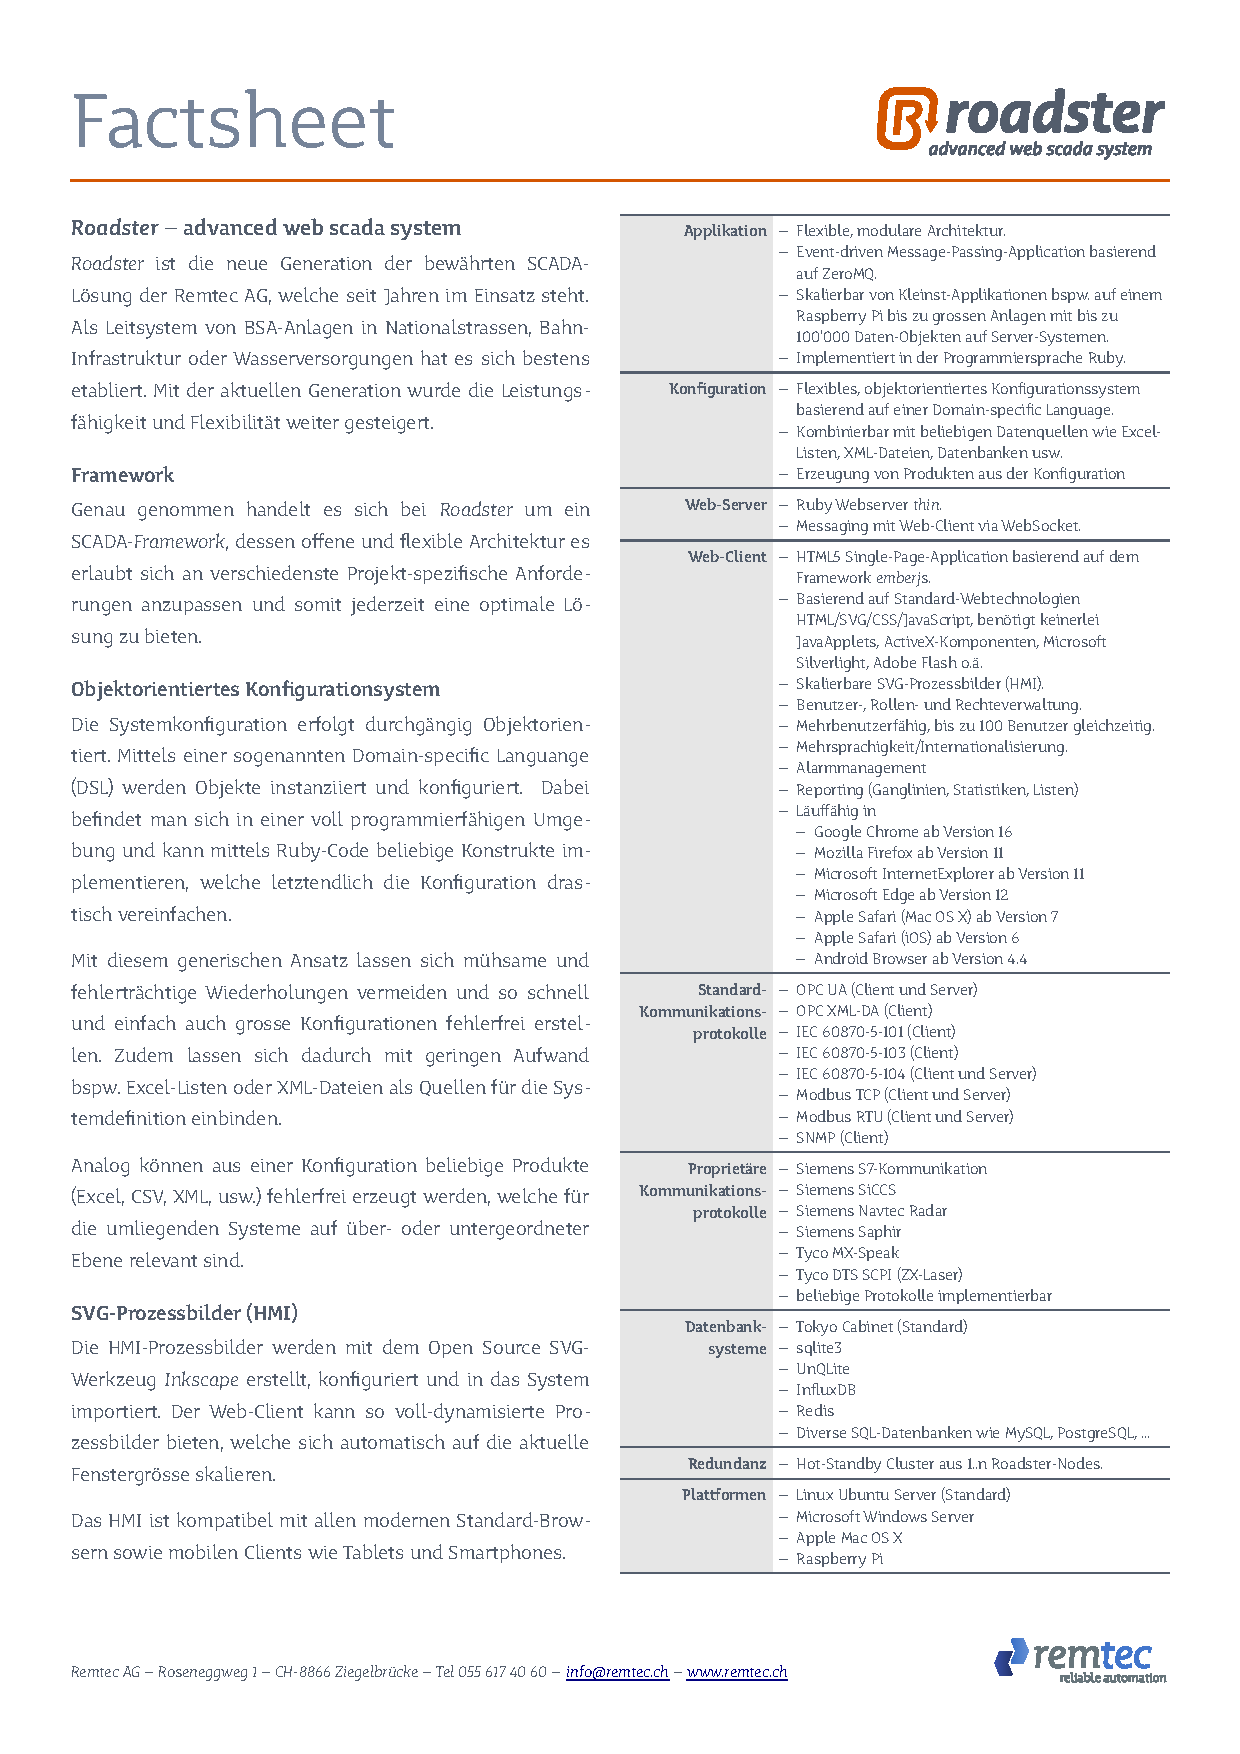
\includegraphics[trim=14.8cm 27cm 1cm 1.4cm, clip=true, width=0.38\textwidth]{img/roadster_factsheet.pdf}\end{raggedright}

\vspace{50mm}
{\scshape\Large Bachelor thesis\\}
\vspace{2cm}
{\huge\bfseries Extension of a SCADA Framework to support High \textls[-150]{A}vailability and Authenticated Encryption\\}
\vspace{1cm}
{\huge\bfseries \#Ruby \#\O{}MQ \#NaCl\\}
\vspace{2cm}
{\Large\itshape Patrik Wenger, Manuel Schuler\\}
\vfill
\begin{center}
\begin{varwidth}{\textwidth}
\begin{description}
	\large
	\item [Client:] mindclue GmbH
	\item [Supervisor:] Prof. Dr. Farhad Mehta
	\item [Expert:] S\"oren Bleikertz
\end{description}
\end{varwidth}
\end{center}
\vfill
% Bottom of the page
{\large September -- December, 2016\\}
\end{titlepage}

%-----------------------------------------------------------------------------
\begin{abstract}
\pagenumbering{roman}

% TODO introduction

% TODO approach and technologies

% TODO result

\end{abstract}
%-----------------------------------------------------------------------------

\chapter*{Declaration of Originality}
We hereby confirm that we are the sole authors of this document, the
described changes to the Roadster framework, and libraries developed as a
byproduct. Unless stated differently, all illustrations in this document are
our creations.

% TODO any usage agreements or license
%\includepdf[width=\textwidth,pages=1,pagecommand=\section{Permissions},trim=1.9cm 3cm 2cm 2cm,clip]{vereinbarung.pdf}

\chapter*{Acknoledgements}
% TODO anyone we'd like to thank

Special thanks to Pieter Hintjens {\textdagger} (3 December 1962 -- 4 October
2016) for his amazing work and contagious passion within the \zmq and
distributed computing communities. We send our deepest condolences to his
family. Rest in peace.

%-----------------------------------------------------------------------------
% TOC, LOF, LOT, LOL
\setcounter{tocdepth}{4}
\tableofcontents
\listoffigures
\listoftables
\listoflistings

\pagebreak
\pagenumbering{arabic}
\setcounter{page}{1}
\setcounter{secnumdepth}{4}

%-----------------------------------------------------------------------------
\part{Management Summary}\label{part:mgmtsummary}
\part*{Management Summary}\label{part:mgmtsummary}
\setcounter{secnumdepth}{0} % avoid section numbering here

\section*{Initial Situation}
TODO describe initial situation, not too technical\\

Roadster is a next generation monitoring application.

\section*{Software Development Process}
TODO describe decision to use RUP/Scrum\\
TODO maybe describe what project management tools we'll be using\\

\section*{Personal Goals}
TODO describe personal goal: the cztop-patterns gem\\

\section*{Project Phases}
TODO describe this phase in retrospection\\

\subsection*{Inception}
TODO include Gantt chart for this phase\\
TODO describe this phase in retrospection\\

\subsection*{Elaboration}
TODO include Gantt chart for this phase\\
TODO describe this phase in retrospection\\

\subsection*{Construction}
TODO include Gantt chart for this phase\\
TODO describe this phase in retrospection\\

\subsection*{Transition}
TODO include Gantt chart for this phase\\
TODO describe this phase in retrospection\\

\section*{Results}
TODO describe results\\


%-----------------------------------------------------------------------------
\part{Technical Report}
% vim: ft=tex
\chapter{Scope}
The technical goals of this bachelor thesis include extending mindclue GmbH's
Roadster framework by adding features such as clustering, high availability and
transport security. This chapter outlines the general scope of this project.

\section{Motivation}
% TODO Why do we care about this thesis? Why are we interested?\\

\subsection*{Backgrounds}
To better understand our motivation, it might help to understand our personal
backgrounds first.

\textbf{Patrik Wenger} did his apprenticeship in computer science at Swisscom
Schweiz AG, and stayed work as a full-time employee for five more years
afterwards. In programming he's most fluent in \gls{ruby} and \gls{c}. During
the winter of 2015/2016, he created \gls{cztop} during leisure time because
there was no good Ruby binding for \gls{zmq}/\gls{czmq} available and a side
project of his demanded it. Fascinated with event-driven programming and
software design patterns such as the \gls{actor-model} (e.g. the
Celluloid\footnote{a concurrency framework for Ruby based on the actor model,
\url{https://github.com/celluloid/celluloid}} library on Ruby, or
Pony\footnote{a young programming language completely based on actors,
\url{http://www.ponylang.org}}, distributed computing and high availability
have long been part of his core interests, especially in conjunction with the
brilliant \zmq library. Having a passion for information security and modern
cryptography\footnote{such as \gls{nacl} or \gls{libsodium} as used by
\gls{zmq}}, especially in this post-Snowden era, this bachelor thesis couldn't
be a better match.

%TODO: Manuel: Javascript, .NET, to expand his horizons
\textbf{Manuel Schuler} did ... and knows and does ... decided to start his own business.
Always keen on learning new things, he did not hesitate to join
this bachelor thesis at the first opportunity.

\noindent
In essence, both students are thrilled to gain more experience in the following
fields and technologies:

\begin{itemize}
	\item Distributed Computing
	\item High Availability
	\item Information Security
	\item \gls{actor-model}
	\item \gls{zmq}
	\item \gls{ruby}
\end{itemize}

\subsection*{Opportunities}
Coming from different backgrounds and having different levels of experience in
each of the above technologies, we can't wait to learn more about them and put
them to actual use. The fact that the product of this bachelor thesis is most
likely going to be used in the real world only adds to the excitement.

This bachelor thesis involves working with Ruby, the Actor Model, \zmq,
distributed computing with high availability, and state-of-the-art
cryptography. Furthermore, in case of successful completion of this thesis, the results will be used in real-world settings like the Ceneri
Base Tunnel. It is a huge opportunity for a solution completely based on free
and open-source software interacting with other industrial systems over open standards. The students, as well as the client, strongly believe
in customized solutions built on reusable, free open-source software.

In addition to that, we look at this bachelor thesis as an opportunity to
become more fluent in English, both written and spoken, as well as to improve
our skills in crafting scientific documents using {\LaTeX}.

Depending on how we perform together as a team, further collaboration might
result in the future, either between the students themselves, or between the
students and the client. Even if our paths will part, this project will
serve as a valuable reference for future job hunting.

Last but not least, we feel like Prof. Dr. Mehta is a respected and competent
teacher whose opinions we highly value. Due to his polite parlance, discussing
project matters, both of the management and the technical kind, has always been
an enrichment.

\subsection{Open-Source engagement}
Getting the chance to use \gls{cztop} and watch it perform definitely adds to
the motivation as well. Its software design has yet to be proven in more
serious settings.

Another personal goal is to create a reusable open-source library as a
byproduct. The intention is that the library makes certain \zmq-based
communication protocols readily available for other developers facing the same
problems.

\section{Initial Situation}

\subsection{mindclue GmbH}
The company mindclue GmbH, located in Ziegelbr\"ucke GL, provides its partner
REMTEC AG with complete \gls{SCADA}\footnote{SCADA software resides in level 2 of the enterprise levels (0--4) modeled by the \gls{isa95} standard, \url{https://en.wikipedia.org/wiki/Enterprise_control}} applications. These are then used to
supervise and control operation and safety equipment found in:
% ISA95 “levels”

\begin{itemize}
\item national freeways, e.g. emergency phones
\item tunnels, e.g. lights and ventilation
\item water supply systems
\item energy facilities
\item many other specialized fields
\end{itemize}

To build these customized applications, their in-house creation
Roadster, a next-generation SCADA framework, is used.

\subsection{Roadster}
Roadster is a SCADA framework written in Ruby. It was, and still
is, developed to produce next-generation SCADA applications to replace legacy
solutions based on its predecessor found in numerous tunnel
facilities in Switzerland.

A Roadster installation combines the following responsibilities:

\begin{itemize}
	\item interaction with subordinate field devices (monitoring \& controlling)
	\item persisting data (e.g. certain sensor data, and events)
	\item sophisticated alarm (\emph{case}) management
	\item providing a machine-to-machine interface to superordinate systems
	\item providing a modern, customized web UI for interaction with operational and executive personnel
\end{itemize}

Among others, the field devices include various kinds of \glspl{PLC}\footnote{an example
is the SIMATIC S7-1500 by Siemens AG,
\url{http://w3.siemens.com/mcms/programmable-logic-controller/en/advanced-controller/s7-1500/Pages/default.aspx}}
as well as emergency call systems\footnote{an example is the NIS ComNode by Trans Data
Management AG,
\url{http://trans-data.com/en/k2-categories/item/149-niscomnode}}.
These are interacted with over numerous propietary and standardized protocols.

\subsubsection{System integration}
This section briefly describes the big picture of Roadster's place within the typical system hierarchy and
relationship with superordinate systems.

Superordinate systems act as clients of a Roadster instance, communicating over
protocols including \gls{SOAP} and \gls{opc-ua}. Their purpose is to
collect and aggregate supervisory information from larger regions. At the top of the
hiearchy are the \gls{FEDRO} (German: \gls{ASTRA}) which combine the information of all
subsystems to provide a nationwide overview.

\begin{figure}[]
	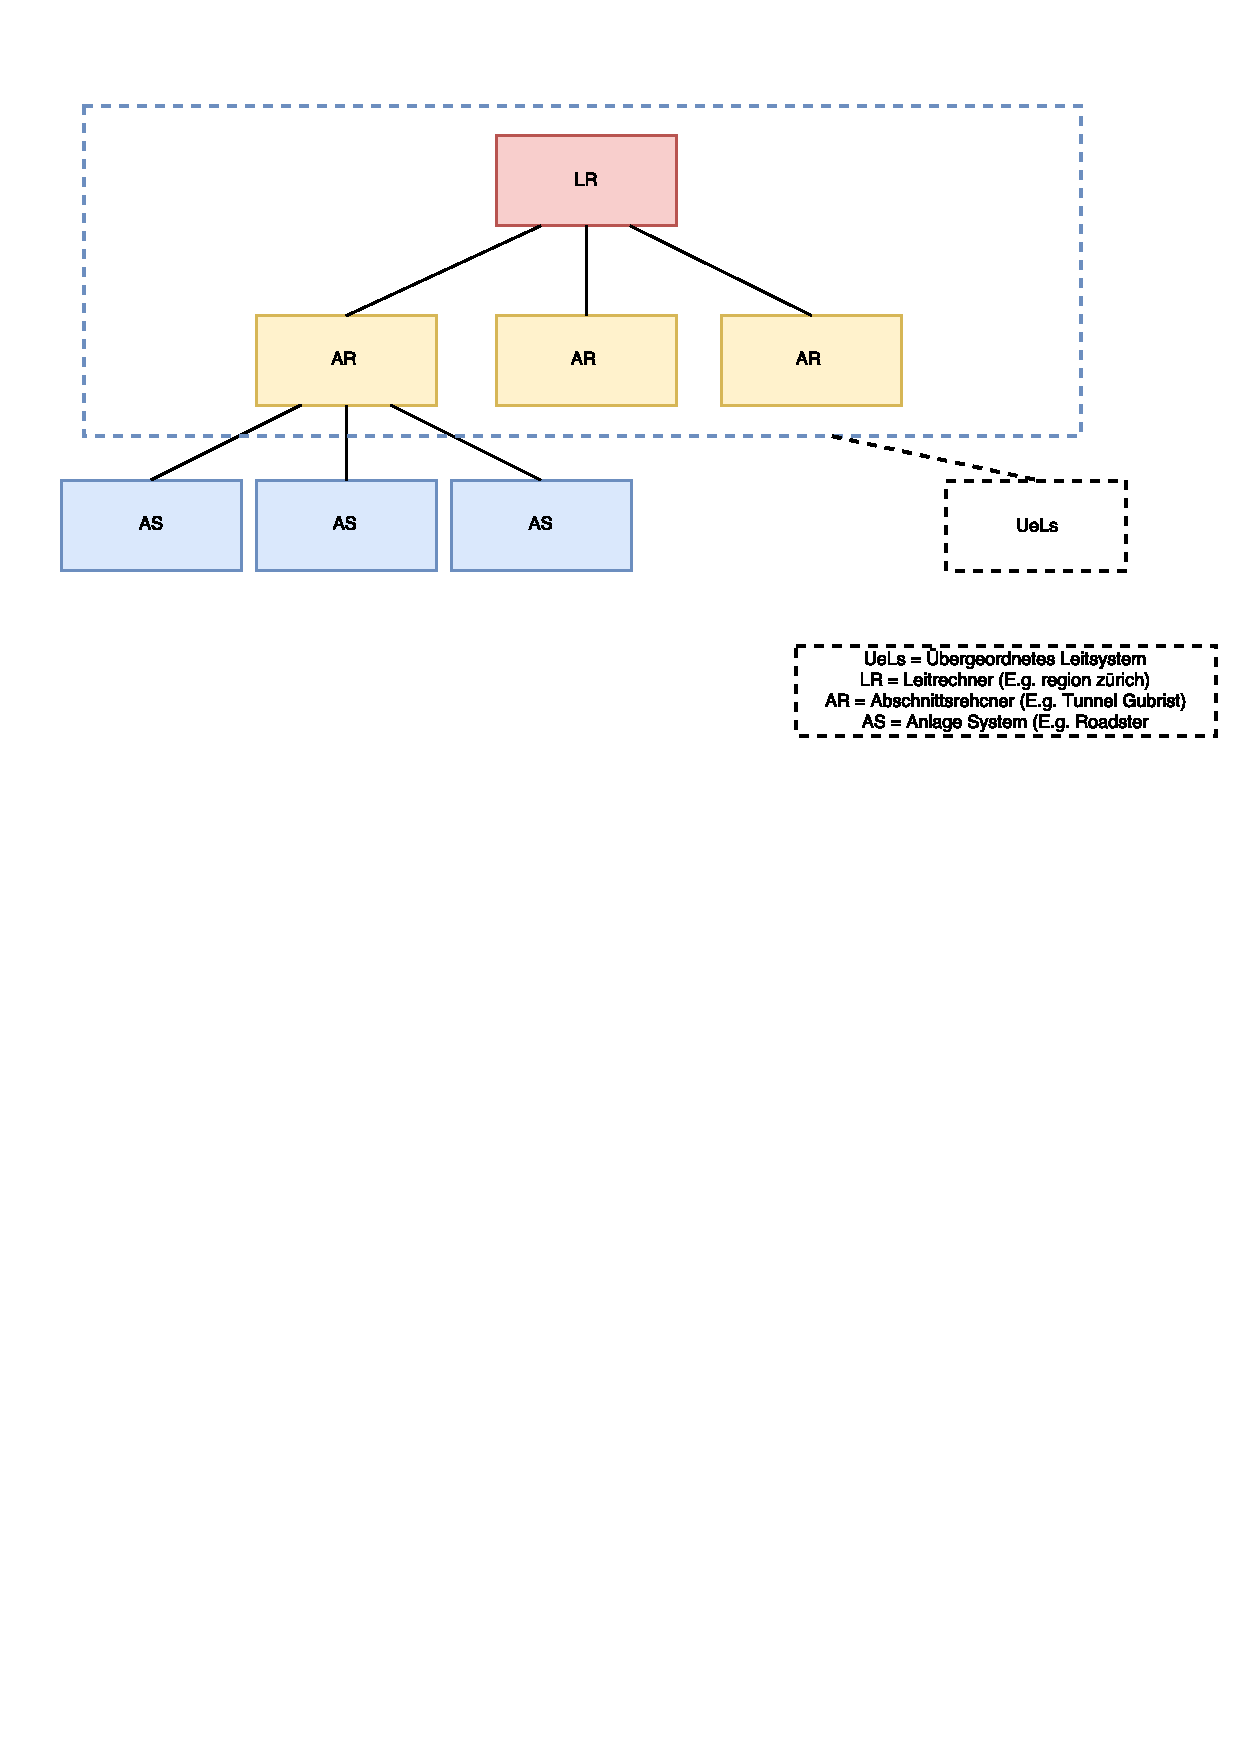
\includegraphics[width=\textwidth]{img/overall_system.pdf}
	\caption{Roadster's place within the overall system}
	\label{fig:roadster:overallsys}
\end{figure}

\autoref{fig:roadster:overallsys} illustrates the overall system. The line
style meanings also apply to the remaining physical topology illustrations. The acronyms
used, which are part of the \gls{FEDRO} terminology, don't have official
English translations; not even the department itself was able to help with
translations on request, so they were left unchanged. A brief description
follows, from the bottom up:

\begin{description}
	\item [ Field devices: ] \hfill\\
	Field devices are various kinds of \glspl{PLC} and other subordinate systems
	used to supervise and control industrial processes. Communication with them
	happens over protocols such as \gls{modbus-tcp}, \gls{iec-104}, and
	\gls{opc-ua}.

	\item [ \gls{AS}: ] \hfill\\
	This is Roadster's domain, or of course the one of another product with similar
	functionality. An AS is responsible for one facility (e.g. emergency call system,
	lighting system, fire alarm system, video monitoring system, ventilation
	system, power supply system, train signaling system).

	\item [ \gls{AR}: ] \hfill\\
	The superordinate system of the collection of all AS found in one larger
	facility such as a tunnel. With the results of this bachelor thesis, this
	\emph{could} be Roadster's domain as well.

	\item [ \gls{LR}: ] \hfill\\
	The superordinate system of the collection of all AR found in a region such as
	Z\"urich. As with AR, this \emph{could} be Roadster's domain as well.

	\item [ \gls{LTA}: ] \hfill\\
	This collective term comprises both the levels of AR and LR. For
	simplicity and readability's sake, this will be referred to as
	\emph{superordinate systems} for the remainder of this document.
\end{description}

\subsubsection{Typical hardware}
Roadster typically runs on entry-level rack server hardware powered by an
Intel\textregistered{} Xeon\textregistered{} processor, or industrial box PCs for smaller systems
commonly used for \gls{IoT} which are powered by more energy efficient processors
such as Intel\textregistered{} Core\textregistered{} and Intel\textregistered{}
Atom\texttrademark{}. The machines are usually equipped with 4 -- 6 GiB of main
memory and Gigabit Ethernet. For reliable systems without any moving parts, one
industrial grade \gls{SSD} or two (in a software \gls{RAID} level 1) setup are used.

\subsection{\zmq}
To understand Roadster's architecture and the rest of this document, it's
helpful to understand the basics of \zmq first. This is a brief introduction to
\zmq for the unfamiliar reader. What follows is a quote from the \gls{zguide}
which does a fairly good job at describing \zmq in a 100 words:

\begin{quote}
``ZeroMQ (also known as \zmq, 0MQ, or zmq) looks like an embeddable networking
library but acts like a concurrency framework. It gives you sockets that carry
atomic messages across various transports like in-process, inter-process, TCP,
and multicast. You can connect sockets N-to-N with patterns like fan-out,
pub-sub, task distribution, and request-reply. It's fast enough to be the
fabric for clustered products. Its asynchronous I/O model gives you scalable
multicore applications, built as asynchronous message-processing tasks. It has
a score of language APIs and runs on most operating systems.  ZeroMQ is from
iMatix and is LGPLv3 open source.''
\end{quote}

Roadster uses \zmq to carry messages between its processes.

For a more detailed introduction, see \autoref{ch:zmq}.

\subsection{Software architecture}
As mentioned earlier, Roadster is event-driven\footnote{\url{https://en.wikipedia.org/wiki/Event-driven_programming}} and built on the Actor model, meaning it exhibits a
shared-nothing architecture. Each Roadster node runs a number of Ruby processes
which communicate via \zmq sockets. The key here is communication:

\begin{quote}
``Don't communicate by sharing state; share state by communicating.''
\end{quote}

Running multiple, loosely coupled processes (actors) allows leveraging the full
potential of modern multi-core processors, while avoiding a whole class of
traditional concurrency problems.

Every Roadster node runs a group of actors:

\begin{description}
	\item [CORE:]\hfill\\
		It is responsible to start the other actors. It also plays a
		key role in keeping state in all actors synchronized, being the
		source of truth.

	\item [COMM:]\hfill\\
		A bunch of COMM actors communicate with the outside world of a
		node. It typically either acts as a client of various kinds of
		subordinate field devices, or as a server to superordinate
		systems. To communicate with subordinate systems, a COMM actor
		utilizes an adapter specifically written for the communication
		protocol in place. The webserver\footnote{The webserver \emph{Thin} is utilized, \url{http://code.macournoyer.com/thin/}} for the web UI also runs in a
		COMM actor.

	\item [STORAGE:]\hfill\\
		This actor is used when information needs to be persisted, such
		as time series or event journals. It's the interface to a
		key-value store.

	\item [LOGGER:]\hfill\\
		This actor collects logging data and sends it to whatever
		target is configured, be it STDOUT, a file, or a syslog server.
\end{description}

\autoref{fig:roadster:arch} illustrates Roadster's architecture.

\begin{figure}[]
	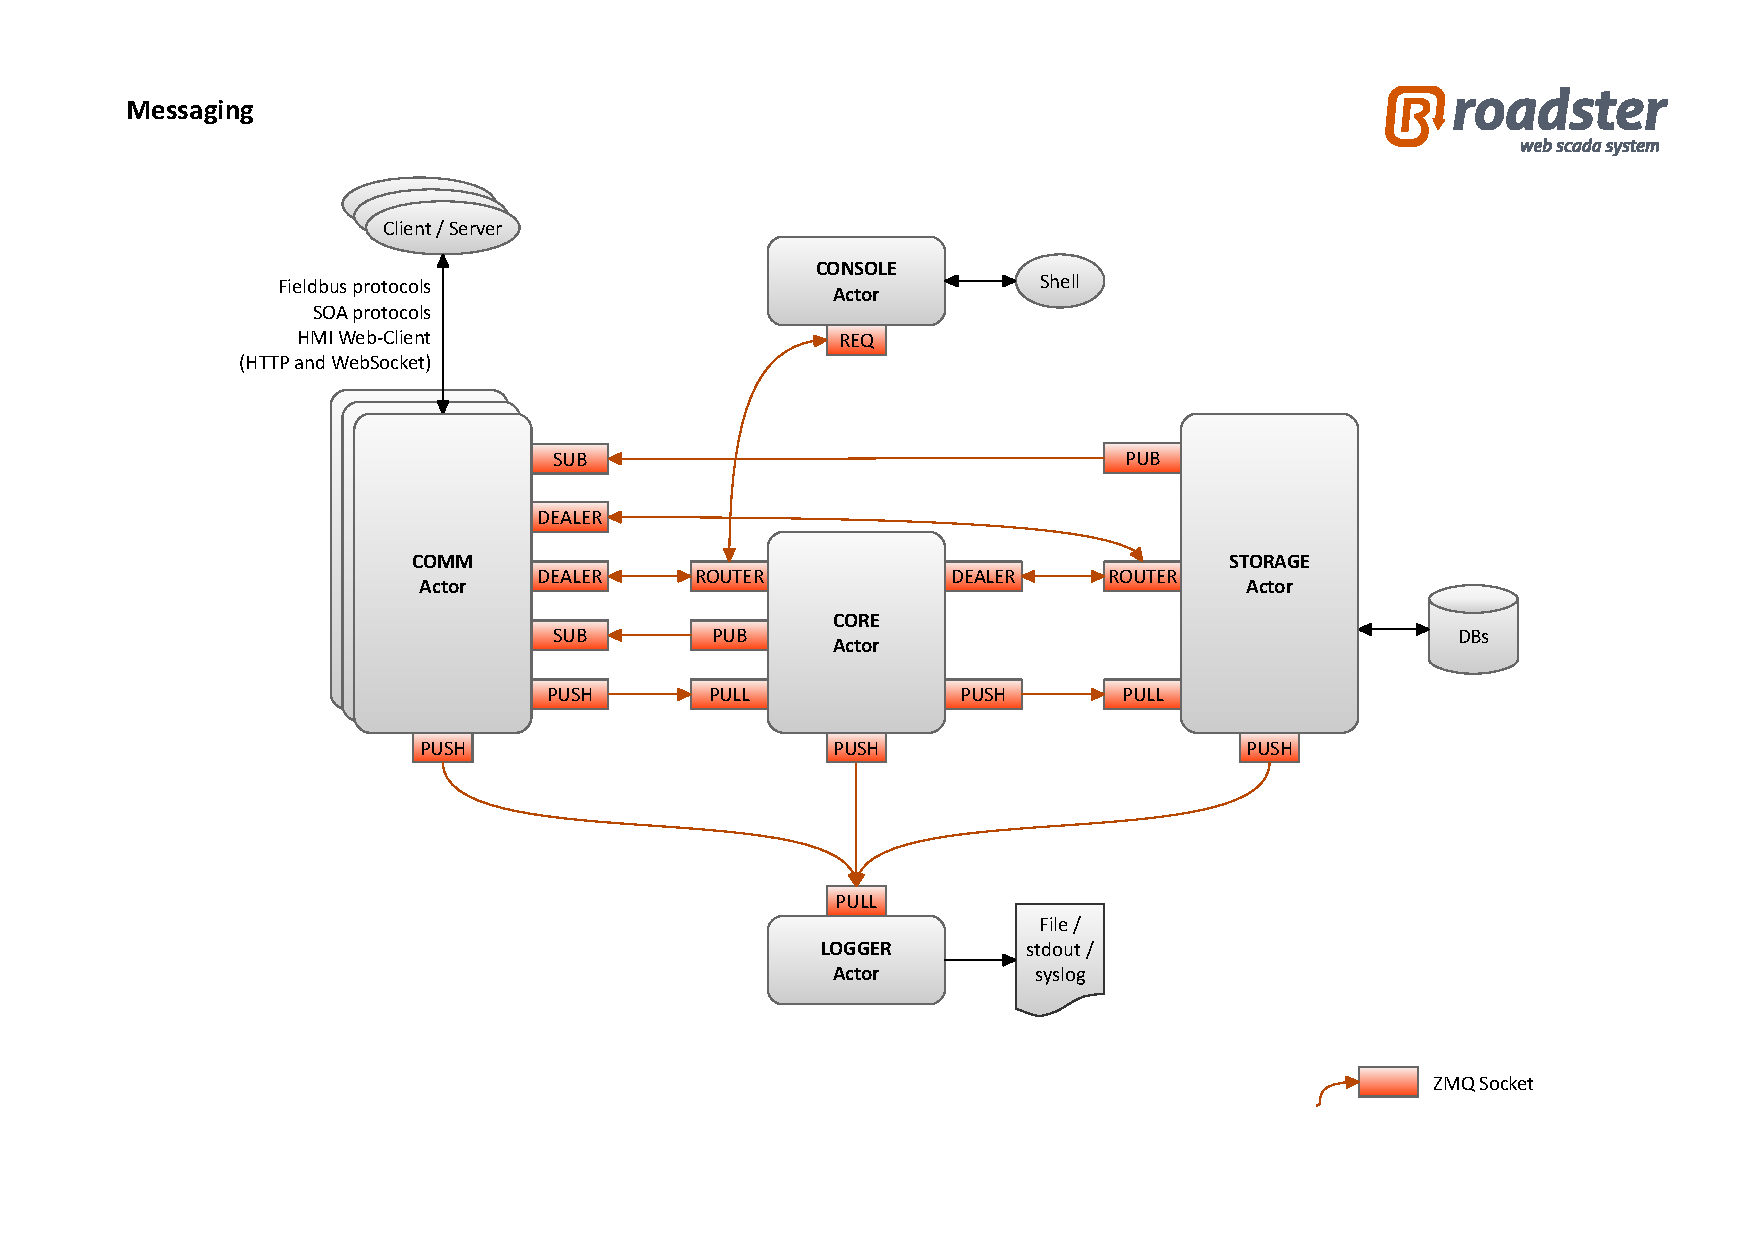
\includegraphics[trim=4cm 2cm 3.5cm 2.8cm, clip=true, width=\textwidth]{img/roadster_arch.pdf}
	\source{Andy Rohr}
	\caption{Roadster's software architecture}
	\label{fig:roadster:arch}
\end{figure}

\subsubsection{Communication Layers}
The communication architecture in Roadster consists of three layers, as
illustrated in \autoref{fig:roadster:layers}. The following list briefly
explains the layers from top (most abstracted) to bottom:

\begin{description}
	\item [Engine layer:]\hfill\\
		Here is the business logic of Roadster, e.g. the \gls{DIM},
		user authentication, adapters for different devices, the web
		\gls{UI}, etc.

	\item [Messaging layer:]\hfill\\
		The \gls{RMP} reside here and implement essential protocols used
		for logging, state synchronization, commands, application controlling,
		and storage. They're explained below in \autoref{sec:rmp}.

	\item [Reactor layer:]\hfill\\
		This layer forms the base, which is where the \zmq sockets and
		\glspl{websocket} are utilized. It is powered by an
		event-loop\footnote{EventMachine is used as a high-performance event-loop to
		manage large numbers of sockets and timers,
		\url{https://github.com/eventmachine/eventmachine}}. Sockets used by COMM actors
		to communicate with various field devices are also integrated into this
		event-loop.
\end{description}

\begin{figure}[]
	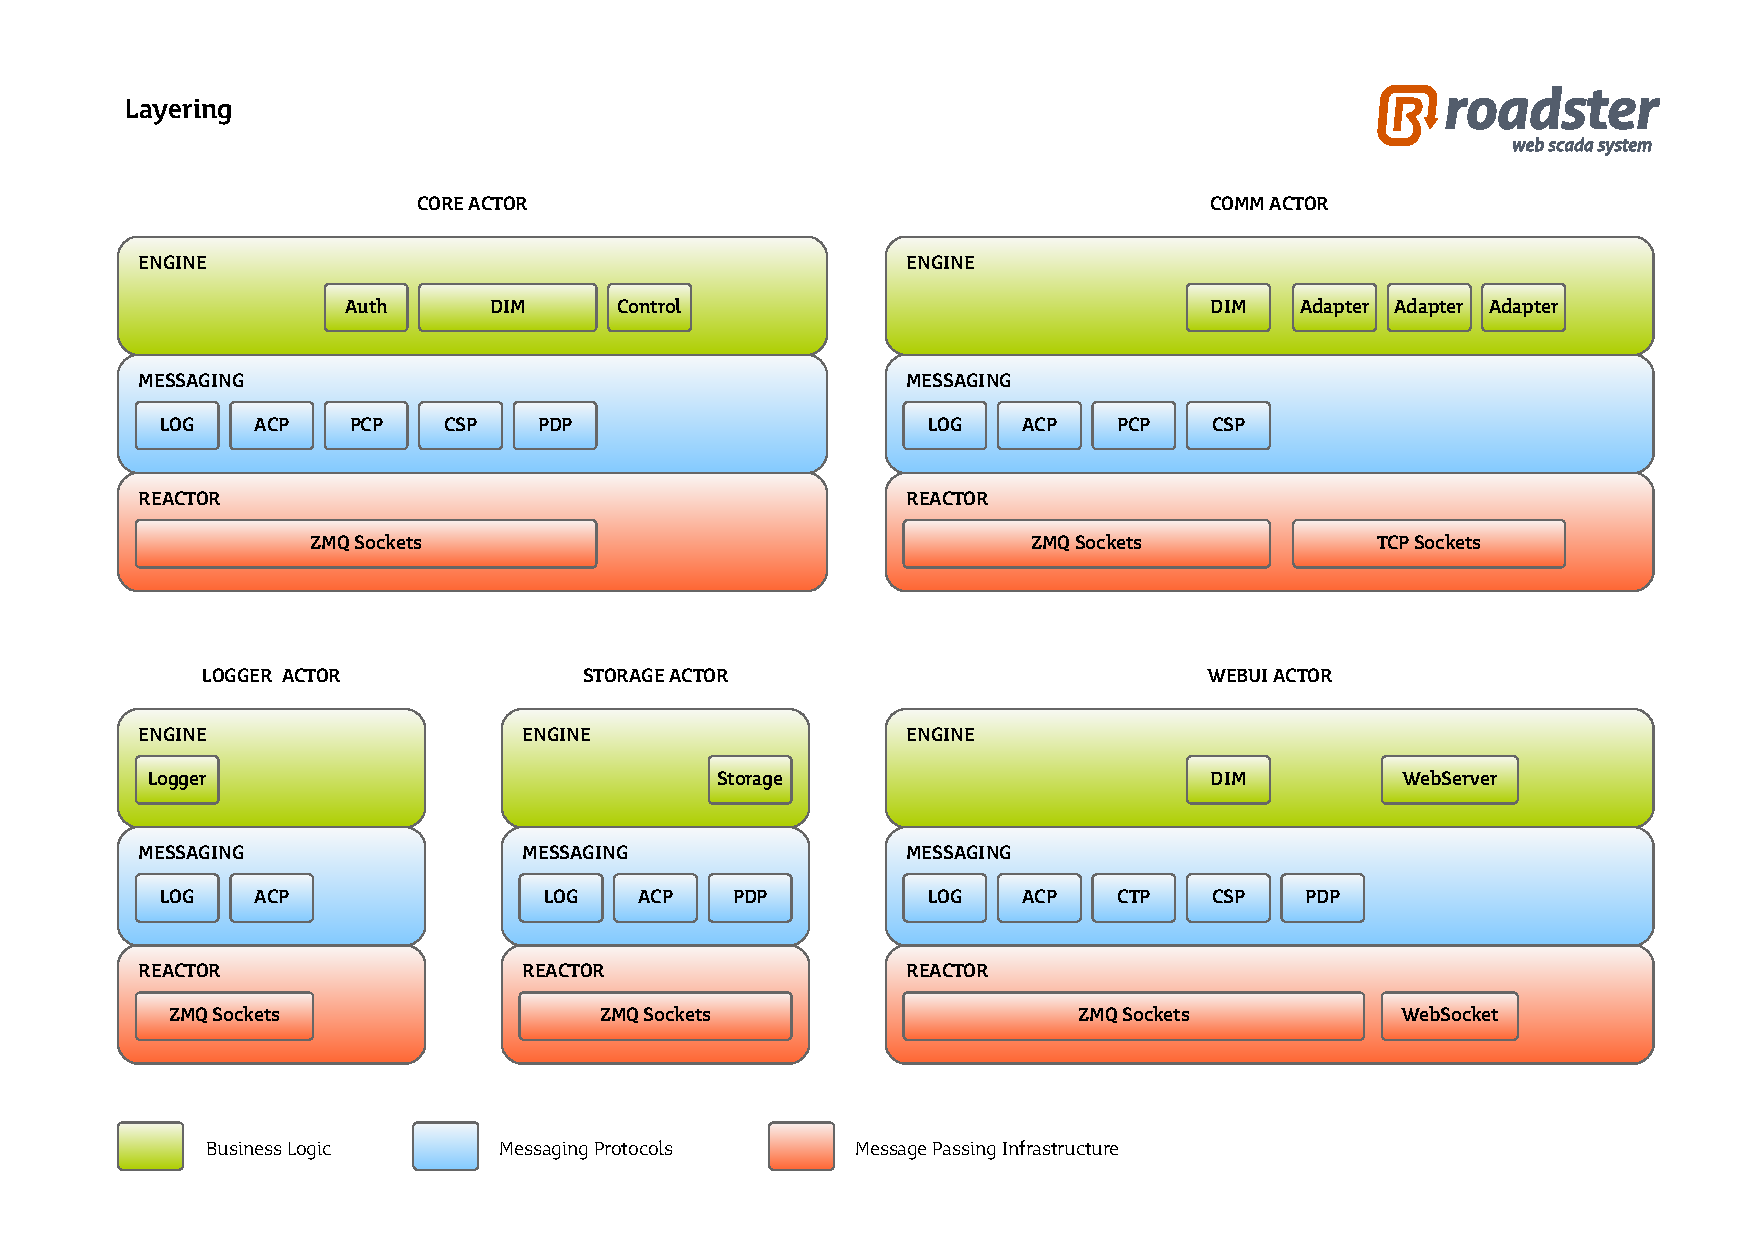
\includegraphics[trim=1.95cm 2.5cm 1.65cm 2.8cm, clip=true, width=\textwidth]{img/roadster_layering.pdf}
	\source{Andy Rohr}
	\caption{Roadster's communication layers}
	\label{fig:roadster:layers}
\end{figure}

\subsubsection{RMP}\label{sec:rmp}
The \gls{RMP} are a collection of protocols implemented and used by Roadster
internally. They reside in the messaging communication layer, and include:

\begin{description}
	\item [\gls{CSP}:]\hfill\\
		Used to synchronize state between the actors.
	\item [\gls{ACP}:]\hfill\\
		Used to control the application state, e.g. shutdown.
	\item [\gls{PDP}:]\hfill\\
		Used when data needs to be persisted.
	\item [\gls{SMP}:]\hfill\\
		Used to suppress the generation of certain \glspl{case}, e.g.
		when a sensor is defect and repeatedly causes cases.
	\item [\gls{PCP}:]\hfill\\
		Used for asynchronous command execution via COMM peers with feedback.
	\item [\gls{LOG}:]\hfill\\
		Used for system logging.
\end{description}

Every actor in Roadster uses a subset of these protocols to perform its job.

Passing messages from actor to actor, which are nothing but serialized Ruby
objects, happens in one of two modes:
\begin{description}
\item [Fire \& Forget:]\hfill\\
No guarantee of correct processing, e.g. DIM updates from COMM to CORE. This
doesn't mean there are no other mechanisms in place to ensure reliability.

\item [Dialog:]\hfill\\
An immediate answer is expected, e.g. when creating a user
session. Sending a message like this looks like it's a synchronous call, even
though it's handled asynchronously under the hood\footnote{This is done by
wrapping the affected code in a Ruby \rb{Fiber}, which is similar to a thread
but allows for cooperative scheduling as opposed to preemtive.} Any protocol
can make use of this primitive.
\end{description}

\subsubsection{DIM}
The \acrfull{DIM} is a tree data structure that lives inside every actor of a Roadster
node. Every actor builds it when starting up by reading the configuration
files. Updates to certain parts\footnote{Namely instances of the meta-model
classes \rb{Case}, \rb{DataItem}, and \rb{Session}} within it are replicated
across all actors. An updated item is marked dirty\footnote{It is marked dirty
by setting its \rb{@lifecycle_state = "updated"}} so it is subsequently synchronized
via the \gls{CSP}. \autoref{fig:roadster:meta-model} is the class diagram of
all the classes whose instances constitute the DIM.

\begin{figure}[]
	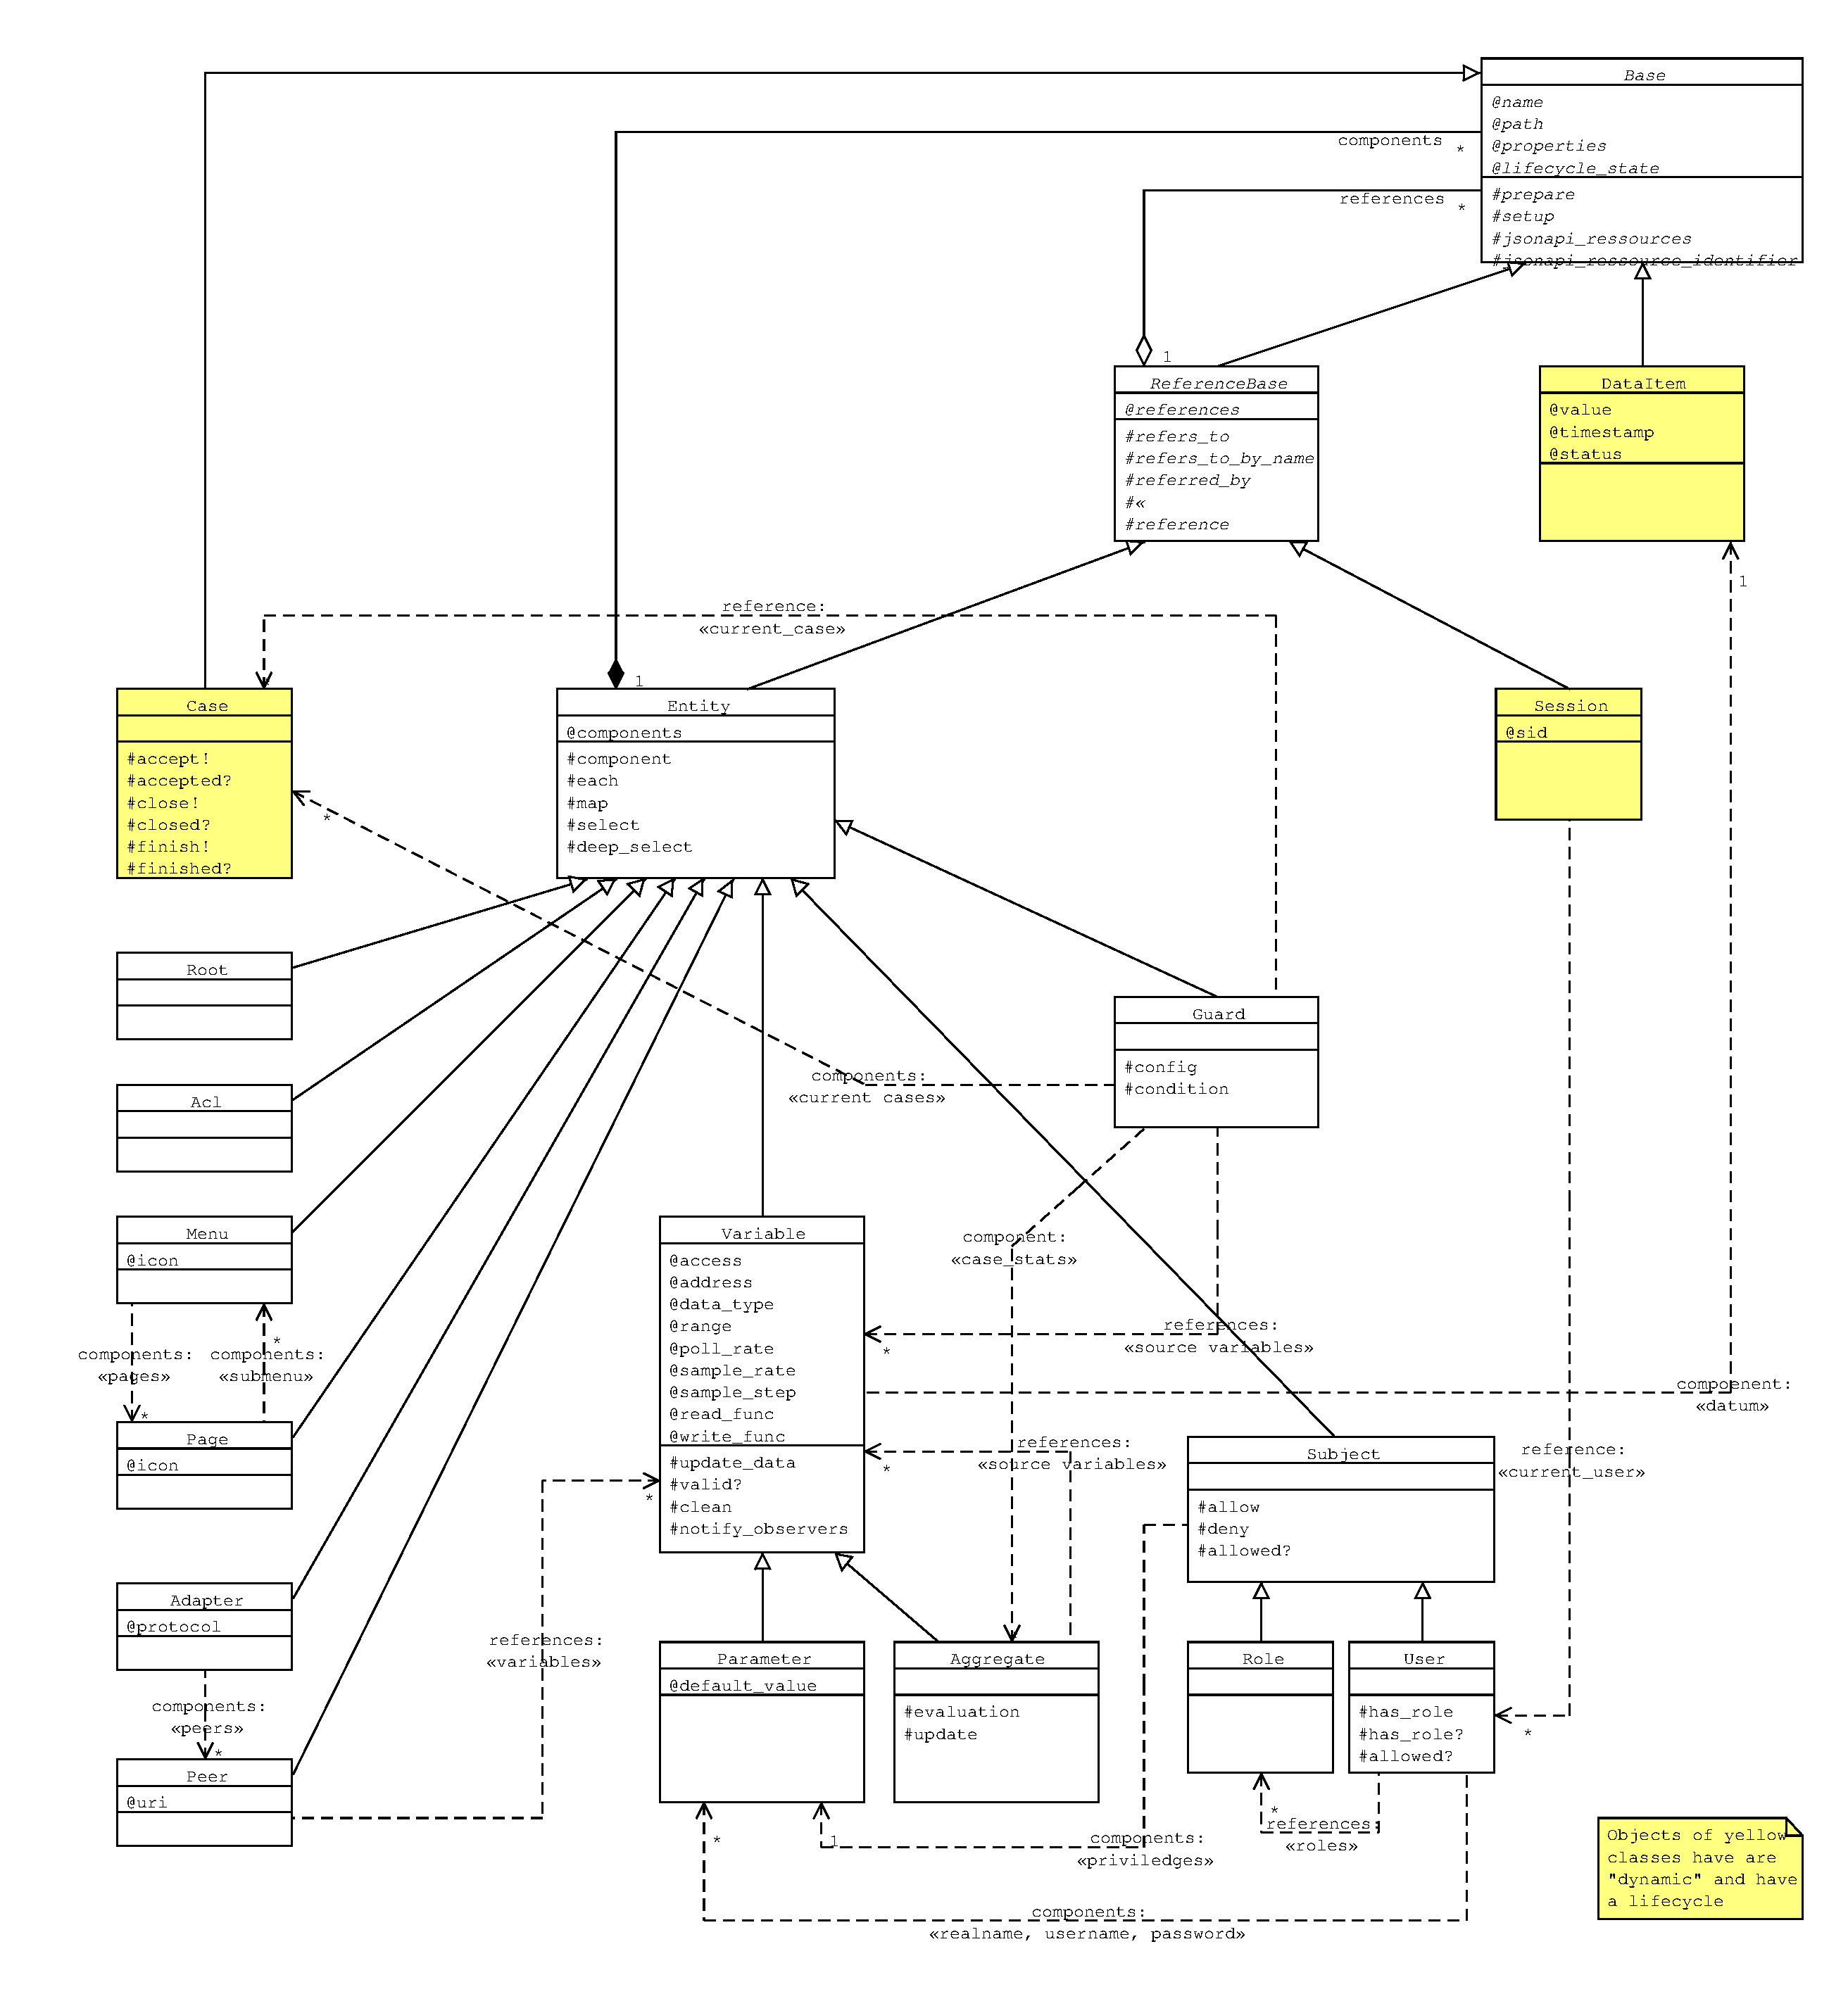
\includegraphics[trim=1.5cm 1cm 1cm 1cm, clip=true, width=0.9\textwidth]{img/meta_model.pdf}
	\source{Andy Rohr}
	\caption{Roadster's Meta Model (used for the DIM)}
	\label{fig:roadster:meta-model}
\end{figure}

\subsubsection{Existing CSP in a nutshell}
\emph{This is a brief introduction/refresher for the Clone State Pattern
implemented by Roadster, which is used for the DIM synchronization. Although Roadster actually sends serialized instances
of CSP message classes to fulfill this protocol, for better readability the
\gls{zguide}'s canonical nomenclature of \gls{clone-pattern} messages will be used.}

The existing \acrfull{CSP} is closely related to the \gls{clone-pattern} from the \gls{zguide}. Its
goal is to keep a state (a list of key-value pairs) in sync across a set of
participants. To greatly reduce the complexity, it's not decentralized: There's
a server part which serves as the single source of truth.

The server uses a ROUTER, a PULL, and a PUB socket; each client a DEALER, a
PUSH, and a SUB socket. The protocol consists of three distinct messages flows:

\begin{description}
	\item [Snapshots:]
		Requesting and receiving the complete, current snapshot of the
		state (all key-value pairs). This happens via a
		ROUTER/DEALER pair of sockets. The request message consists solely of
		the humorously named ICANHAZ command. The response is the
		complete set of KVSET messages so a late-joining (or previously
		disconnected) client can rebuild the current snapshot.

	\item [Upstream updates:]
		Updates always originate from clients and are sent to the
		server via a PUSH/PULL pair of sockets. These are KVSET messages.

	\item [Downstream updates:]
		After being applied to the server's copy of the state,
		updates get a sequence number and are published back to all
		clients. This happens via the PUB socket and
		uses KVPUB messages.
\end{description}

By making all updates go through the server, a total order is enforced,
which is crucial to keep the state consistent across all clients.

To avoid risking a gap between requesting the current snapshot and subscribing
to updates, a client actually subscribes to the updates first, then gets the
snapshot, and then starts reading the updates from the socket (which has been
queueing updates in the meantime, if any). Updates that are older or the same
age as the received snapshot are skipped, and only successive updates are
applied (tested by comparing the sequence numbers).

Because message loss via the third message flow (PUB-SUB) is unlikely but
theoretically possible, the client checks for gaps in the sequence number of
each KVPUB message. If a gap is detected, the current state is discarded and a
complete resynchronization happens. This is brutal, but is very simple and thus
robust; there's no complexity that would leave room for nasty corner cases.

Keys can be treated hierarchically (e.g. \sh{topic.subtopic.key}) and thus, a
client can optionally subscribe to only a particular subtree. This is useful
when the number of client grows and not all of the state needs to be on every
client. In that case, the topic of interest is sent by the client along with
the ICANHAZ message.


\section{Goals}
% TODO preprocessed mandatory goals\\
% TODO retrospective, diff with initial goals\\

To summarize the mandatory goals from the Task Description in \autoref{ch:task-desc}:

\begin{enumerate}
	\item Getting familiar with Roadster
	\item Extending the communication protocols to support clustering
	\item Extending the communication protocols to add high availability
\end{enumerate}

The optional goals are:

\begin{enumerate}
	\item Encryption of the communication
	\item Providing of the highly available \gls{opc-ua} server interface
\end{enumerate}

Secure inter-node communication within a Roadster cluster is important to
mitigate common security concerns with SCADA systems which are becoming more
and more open due to standardization. To quote wikipedia:

\begin{quote}
``In particular, security researchers are concerned about:
	\begin{itemize}
		\item the lack of concern about security and authentication in the design, deployment and operation of some existing SCADA networks
		\item the belief that SCADA systems have the benefit of security through obscurity through the use of specialized protocols and proprietary interfaces
		\item the belief that SCADA networks are secure because they are physically secured
		\item the belief that SCADA networks are secure because they are disconnected from the Internet.''
	\end{itemize}
\end{quote}

% vim: ft=tex
\chapter{Requirements}\label{ch:reqs}
The requirements gathered during the first and second meeting with the client are
explained in this chapter. These are more concrete than the ones listed in the
original task description in \autoref{ch:task-desc}.

First of all, these are the client's priorities:

\begin{enumerate}
\item Federation functionality, namely:
	\begin{enumerate}
		\item Topology definition
		\item DIM replication
		\item Message routing
	\end{enumerate}
\item \Gls{HA}
\item Persistence replication
\item Encryption (optional)
\item DIM access control
\item OPC UA \gls{HA} (optional)
\end{enumerate}

The following sections explain the requirements in greater detail, starting
with the functional ones. The non-functional requirements are described in
\autoref{sec:nfr}.

The functional requirements are each described in prosa as understood by the
students first and then formally in \gls{gherkin} style features. Those feature
specifications will later be useful to deduce test cases.

\section{Federation}
% TODO: big picture
Roadster will need to be run on multiple nodes in a hierarchical topology,
forming a distributed computing architecture. The root node would then act as
the client-facing server. This is formally specified in
\autoref{lst:feature:federation}. Typical node topologies include:

\begin{description}
	\item [ Single level with a single node: ] \hfill\\
		This is the legacy setup and is what Roadster is already able
		to do. It consists of a single node. This is illustrated in
		\autoref{fig:topo:sl:noha}, where the single node is denoted as node R.

	\item [ Multi level: ] \hfill\\
		This is the most basic federation setup. There is a root node, and
		a number of subnodes. Each subnode is directly connected to a number of field devices such as
		\glspl{PLC} or emergency phones. This is illustrated in
		\autoref{fig:topo:ml:noha}, where the root node is denoted as R
		and the subnodes as S1, S2, and S3.
\end{description}

\begin{figure}[]
	\center
	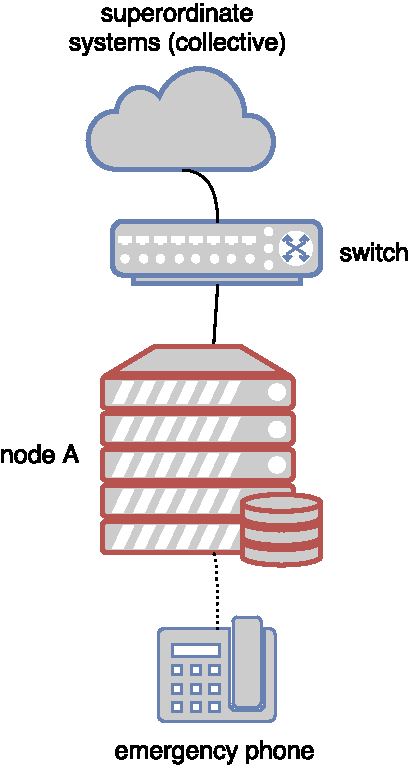
\includegraphics[width=0.2\textwidth]{img/topo_sl_noha.pdf}
	\source{mindclue GmbH}
	\caption{Logical federation topology example: Single level with a single node (legacy)}
	\label{fig:topo:sl:noha}
\end{figure}
\begin{figure}[]
	\center
	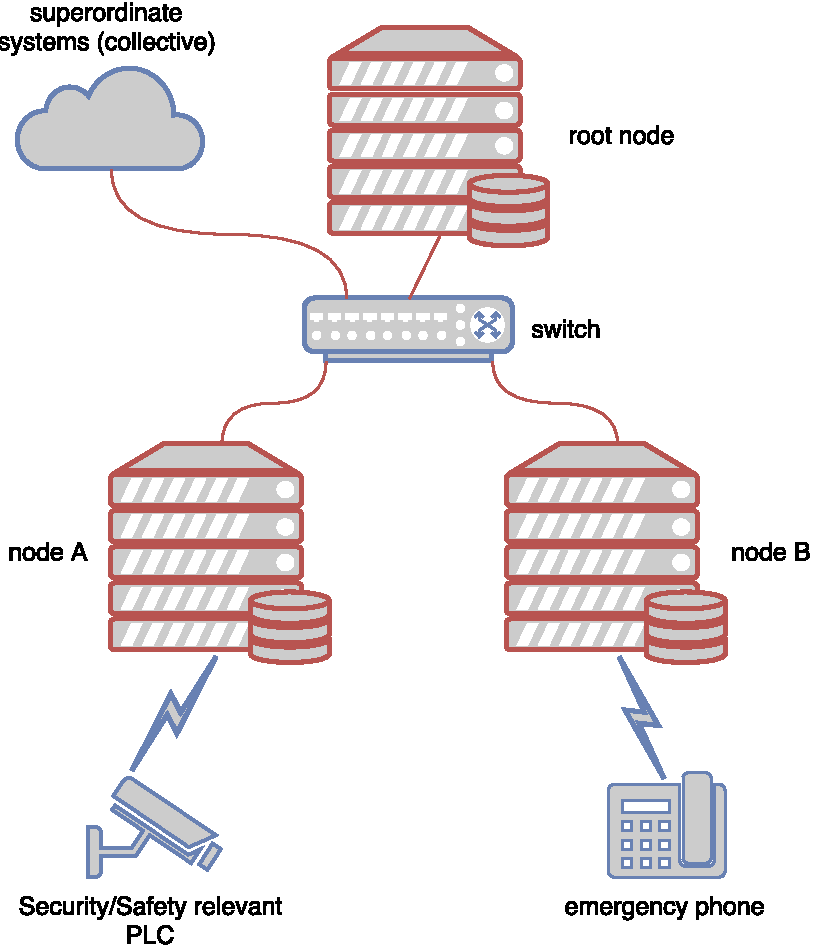
\includegraphics[width=0.6\textwidth]{img/topo_ml_noha.pdf}
	\source{mindclue GmbH}
	\caption{Logical federation topology example: Multi level}
	\label{fig:topo:ml:noha}
\end{figure}

% TODO: features are not listings
\begin{listing}
	\inputminted{Gherkin}{listings/features/federation/federation.feature}
	\caption{Formal feature: Federation}
	\label{lst:feature:federation}
\end{listing}

\paragraph{Network infrastructure} Roadster nodes would typically be connected
through a network switch, possibly assigned their own \gls{VLAN}. The root node
would typically have two \glspl{NIC}: One connected to the processing network,
i.e. the Roadster federation, and another one connected to the client network.

\subsection{DIM extension}

\subsubsection{Replication}
Extending the \gls{CSP} to keep the \gls{DIM} consistent across all nodes is a central
part of the federation functionality. This demands a replication of all modifications to
the dynamic subset of DIM objects to all other nodes in the federation.

\paragraph{Bidirection} Just like the CSP, bidirectional replication is required.
Because every node is authorative for its subset of objects in the
DIM, every node has to replicate modifications that have happened in the
meantime to its direct peers nodes, no matter if these peer nodes are
supernodes or subnodes.

According to the meta model in \autoref{fig:roadster:meta-model}, these dynamic
objects are exactly the instances of one of the following three
classes (marked yellow in the class diagram):
\begin{itemize}
	\item \sh{Roadster::Domain::Model::DataItem}
	\item \sh{Roadster::Domain::Model::Session}
	\item \sh{Roadster::Domain::Model::Case}
\end{itemize}

As described earlier, instances of these entity classes are marked "dirty" when
modified until they are replicated.

\subsubsection{Access control}
The aforementioned requirements imply that modifications to the \gls{DIM} can only be done by the
owning node. A node
must not modify objects owned by other nodes directly. This is to ensure that each node is its own source of truth
% FIXME: source of truth == ?
to all other nodes in the federation. Only the owner node can enforce a single
sequence of updates to its part of the DIM, which is necessary to guarantee
eventual consistency \cite[Chapter 5, Reliable Pub-Sub (Clone Pattern), Republishing
Updates from Clients]{zmq:zguide} across all actors of all nodes.

These two aspects to the DIM extension are formally specified in \autoref{lst:feature:federation:dimsync}

\begin{listing}
	\inputminted{Gherkin}{listings/features/federation/dim_extension.feature}
	\caption{Formal feature: DIM replication}
	\label{lst:feature:federation:dimsync}
\end{listing}

\subsection{Autonomy}
It is important that every node (and its subnodes) can keep up the operation autonomously even if the
link to its supernode fails or the supernode itself fails. This means that updates to
the \gls{DIM} must be possible even when neighboring nodes (including the supernode) are unavailable. After the
recovery from the outage, the \gls{DIM} replication shall be reinitiated so
all pending updates are shared to all other nodes as per normal operation.

This is formally specified in \autoref{lst:feature:federation:autonomy}.

\begin{listing}
	\inputminted{Gherkin}{listings/features/federation/autonomy.feature}
	\caption{Formal feature: Autonomy}
	\label{lst:feature:federation:autonomy}
\end{listing}

\subsection{Message routing}
There needs to be a message routing mechanism so a user
of one node's web UI can send a command (passed as a message) to another node where it will be
executed. An example for this is a forced value in the DIM to ignore the
actually measured value reported by a device in case the device is known to be
wrong. The common case where the command is issued at a higher level in the node
topology is priority. E.g. in a multi level setup with a root node R and two
subnodes S1 and S2, issuing a command on S1 for S2 has a low priority.

This is formally specified in \autoref{lst:feature:federation:cmdrouting}.

\begin{listing}
	\inputminted{Gherkin}{listings/features/federation/message_routing.feature}
	\caption{Formal feature: Message routing}
	\label{lst:feature:federation:cmdrouting}
\end{listing}

\section{High availability}
Roadster must be able to run in certain high availability setups. Achieving
this is done by adding redundant Roadster nodes.

The following additional federation topologies must be supported:
\begin{description}
	\item [ Single level \gls{HA}: ] \hfill\\
		This is when there are exactly two nodes, both of them
		connected to the same set of field devices. The difference to a
		non-redundant case is the added backup node, forming a HA
		cluster. The field devices are thus connected to the HA cluster
		using two redundant paths. Both HA peers are able to interact
		with the field devices to perform operation tasks (e.g. reading
		sensor data, writing down configurations), but only one of them
		(the active one) must do so. This is illustrated in
		\autoref{fig:topo:sl:ha}.

	\item [ Multi level, \gls{HA} at root only: ] \hfill\\
		There can be multiple hierarchy levels within a Roadster federation, such as two or
		three (anything else is declared out of scope of this thesis). Introducing
		redundancy is done at the root level in the form of a HA
		cluster, consisting of a primary and a backup node. An example of this setup is illustrated in
		\autoref{fig:topo:ml:ha}.
\end{description}

\begin{figure}[]
	\center
	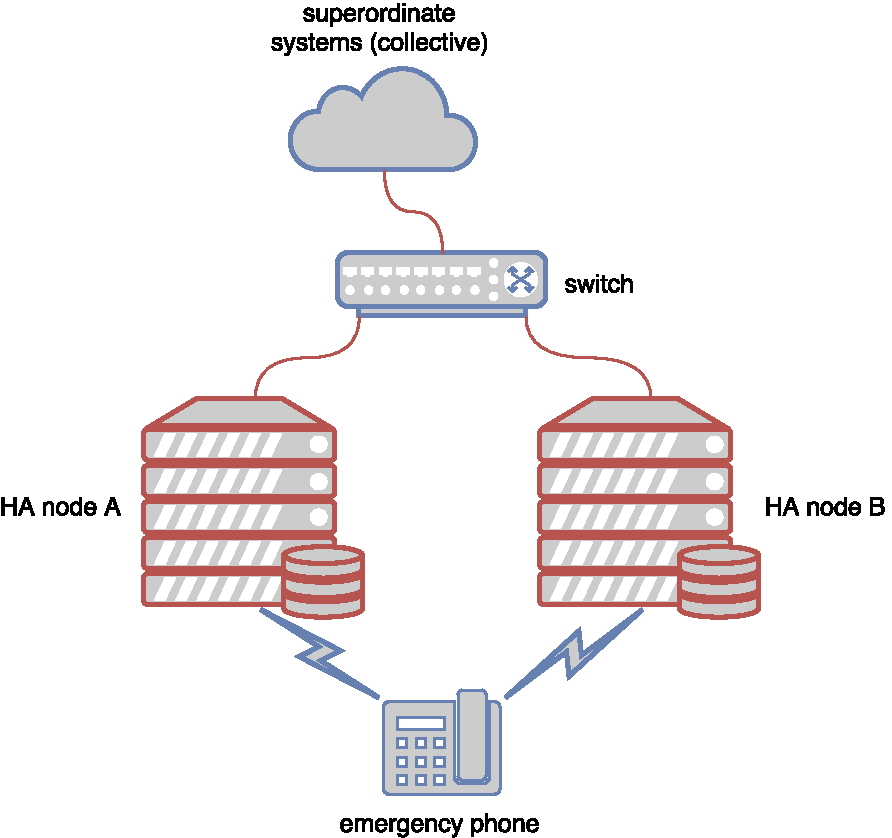
\includegraphics[width=0.5\textwidth]{img/topo_sl_ha.pdf}
	\caption{Federation example: a HA cluster and redundantly connected field devices}
	\label{fig:topo:sl:ha}
\end{figure}
\begin{figure}[]
	\center
	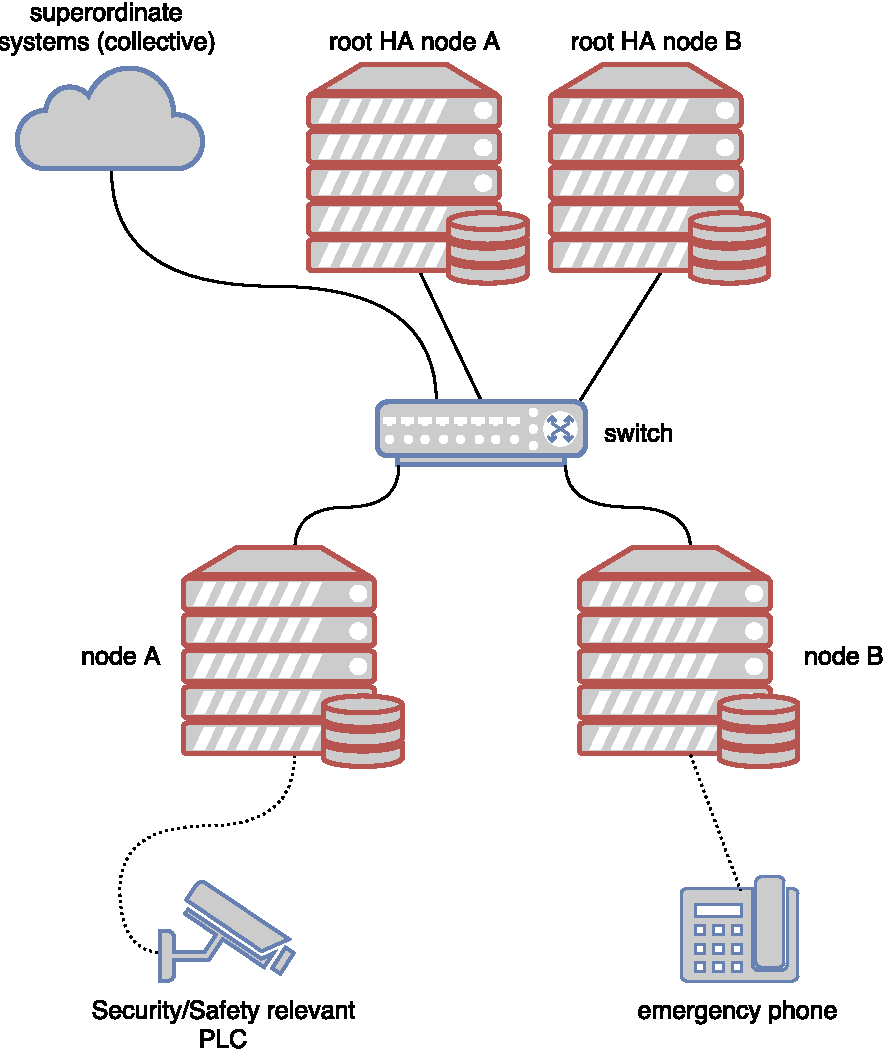
\includegraphics[width=0.5\textwidth]{img/topo_ml_ha.pdf}
	\caption{Federation example: HA cluster at root, two subnodes, each with field devices}
	\label{fig:topo:ml:ha}
\end{figure}

The following topologies are unusual, not planned for, and are thus declared
outside the scope of this thesis; however, they should be kept in mind so a
future extension to support them is feasible:

\begin{description}
	\item [ Multi level, \gls{HA} at bottom: ] \hfill\\
	A single root node at the top and a subordinate HA pair each connected
	to the same field device.

	\item [ Multi level, \gls{HA} in the middle: ] \hfill\\
	A single root node at the top, a subordinate HA pair, which in turn has
	a subordinate node connected to some field device.
\end{description}

\begin{figure}[]
	\center
	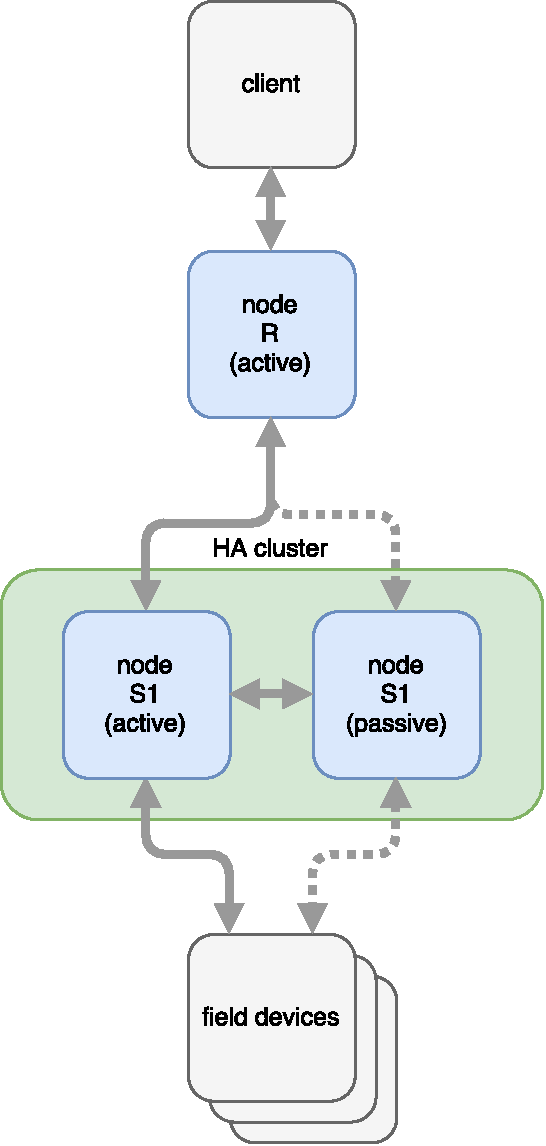
\includegraphics[width=0.5\textwidth]{img/ml_ha_on_sub_exotic_topology.pdf}
	\caption{Unusual federation example: Multi level, \gls{HA} at bottom}
	\label{fig:topo:exotic:ml:ha:on:sub}
\end{figure}

\begin{figure}[]
	\center
	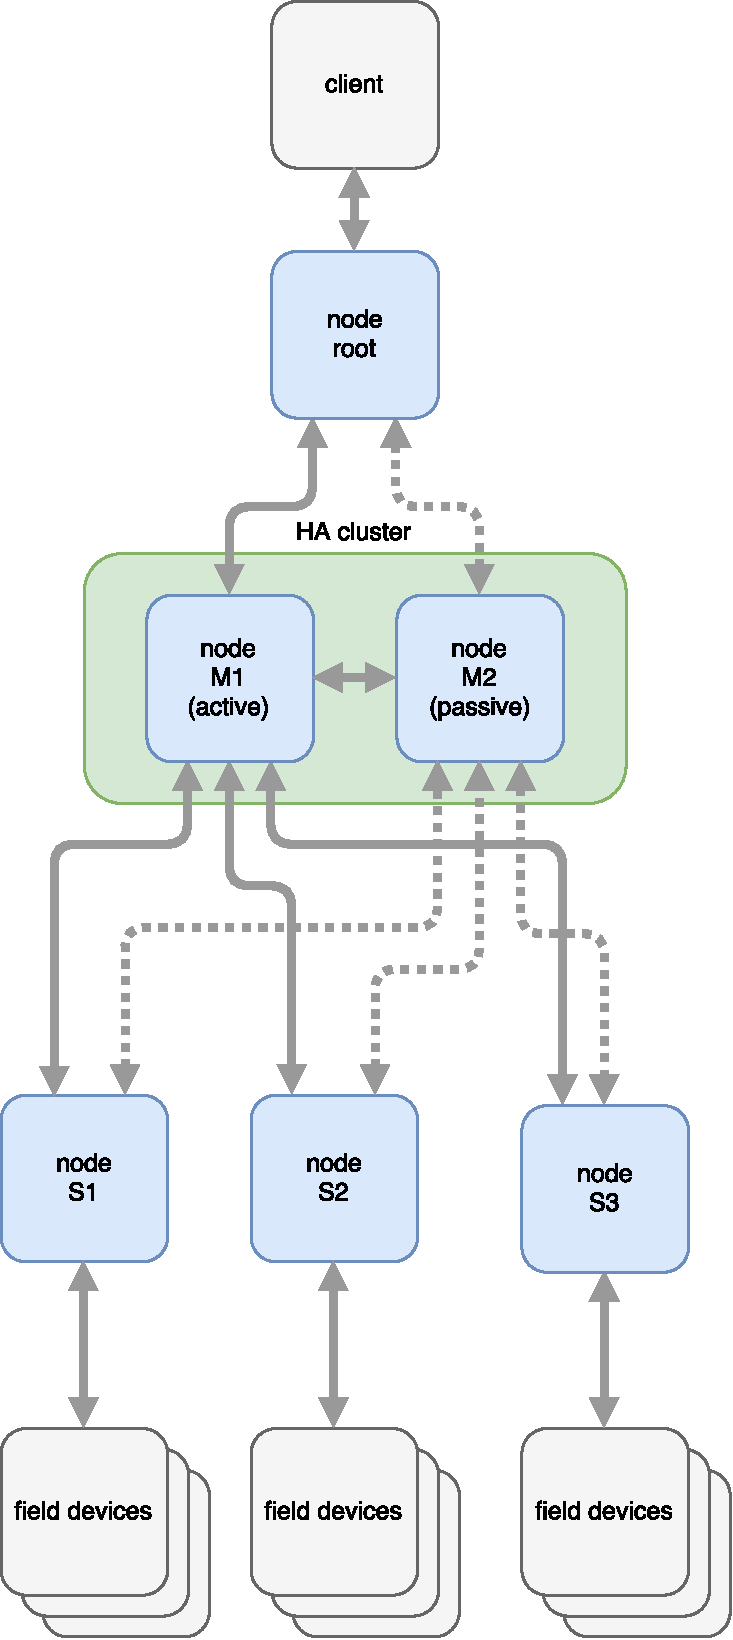
\includegraphics[width=0.5\textwidth]{img/ml_ha_on_mid_exotic_topology.pdf}
	\caption{Unusual Federation example: Multi level, \gls{HA} in the middle}
	\label{fig:topo:exotic:ml:ha:on:mid}
\end{figure}


\paragraph{Dedicated network link}
It is possible that there will be a dedicated, direct network link from one peer to
the other. However, this will not be the typical case.

\paragraph{Split-brain syndrome}
At initialization, the two peers must be able to automatically decide on which peer
becomes active first.  At any time, only one of the two HA peers must be
active (i.e. serving clients), and the other one must stay passive (i.e. ignore
client requests and only keep its DIM up-to-date). The passive HA peer shall
take over in the event that the currently active peer becomes unavailable.
Measures must be taken to avoid the dreaded split-brain syndrome where both HA
peers become active.

The types of failures that need to be handled include:
\begin{itemize}
	\item Software failure on the primary node, like an application or OS crash
	\item Hardware failure on the primary node, like a defect power supply
	\item Failure of a network link, completely disconnecting a HA peer from the federation
\end{itemize}

All three failure types listed can collectively be called \emph{crash},
as their effects are the same from the point of view of the whole federation.

The high availability requirement is formally specified in \autoref{lst:feature:ha}

\begin{listing}
	\inputminted{Gherkin}{listings/features/high_availability.feature}
	\caption{Formal feature: High availability}
	\label{lst:feature:ha}
\end{listing}

\section{Persistence replication}
% TODO: explain what south/north means, maybe in scope already
This is about the replication of persisted data, which is currently stored
in \gls{tc} databases on a Roadster node, one for each kind of data. With the federation functionality, this is
still true: Every node will have its own set of key-value stores. Changes to the persisted
data must flow from south to north (towards the root node), so the root
node can collect and maintain a replication of the persisted data of all
nodes within the federation, recursively.

Again, it is important that every node and its subnodes form an autonomous subsystem. So
in case the link to its supernode fails, it has to continue working. As soon as
the link is repaired, replication of the delta (changes to the data) can
be initiated.

This is different from \gls{DIM} replication, as the DIM is shared across
all nodes and is a relatively small data structure holding merely the current state. The \gls{tc} databases
can possibly contain large amounts of data (in the hundreds of megabytes) and
are shared only towards the root node (thus "bubbling up").

This is formally specified in \autoref{lst:feature:persistence_synchronization}.

\begin{listing}
	\inputminted{Gherkin}{listings/features/persistence_synchronization.feature}
	\caption{Formal feature: Persistence replication}
	\label{lst:feature:persistence_synchronization}
\end{listing}

% ---------------------------------------------------------------------------
\section{Non-functional requirements}\label{sec:nfr}
The following subsections elaborate on the non-functional requirements.

\subsection{Simplicity}
The two reoccuring patterns that surfaced during the requirements gathering
meeting were:

\begin{enumerate}
\item \gls{KISS} principle. Simplicity is favored, as experience shows that
	simpler systems are more stable, so complexity should be avoided if not
	absolutely necessary.

\item No premature optimization since it is the root of all evil.\footnote{Quote
	by Donald Knuth: ``Premature optimization is the root of all evil.''}
\end{enumerate}
% TODO: recycle ZMQ sockets


\subsection{Testing}
Regarding testing, the following requirements exist:
\begin{itemize}
	\item the student's contributions are verified using unit tests
	\item the formally described scenarios shall be verified using
		integration tests in a close-to-reality setup, either
		automatically or manually
\end{itemize}

\subsection{Constraints for persistence replication}
100\% consistency is not an absolute requirement for persistence replication.
Nor is zero data loss an absolut requirement. However, it is mandatory that
updates make it to the root node within 30 seconds.

\subsection{High availability for OPC UA}
The high availability feature shall be designed with \gls{opc-ua} in mind. It
should be easy to adapt it to the various kinds of server redundancies specified
in OPC-UA, including the transparent and non-transparent variants.

\subsection{Encryption}
\emph{This is optional. Also, this requirement has the lowest priority not
because it is insignificant, but because it is trivial to enable transport level
security on \zmq sockets later on.}

The inter-node communication of a Roadster federation must be secured using
encryption. Recent versions of \zmq offer modern, authenticated encryption,
including server and client authentication (the latter is optional).
The client favors a solution where every communication partner (a node)
authenticates all its communication partners, and vice versa.

Since the \zmq binding used in the legacy version is unmaintained and does not
allow encryption, it has to be exchanged with a more appropriate library.

\subsection{Code style}
The coding guidelines desired by the client are basically the ones written down
in the popular Ruby style guide \cite{rb:style-guide}, with the following
differences or special remarks:

\begin{itemize}
	\item Non-interpolated strings shall be written as \rb{'foobar'}, not \rb{"foobar"}.

	\item Method invocation: Parenthesis shall be omitted when unnecessary, even with
		arguments present. This is opposed to the rule
		\cite[\href{https://github.com/bbatsov/ruby-style-guide\#method-invocation-parens}{Method~Invocation~Syntax}]{rb:style-guide}.

	\item Method definitions shall be preceded by two blank lines. This slightly
		extends the rule
		\cite[\href{https://github.com/bbatsov/ruby-style-guide\#empty-lines-between-methods}{Source~Code~Layout}]{rb:style-guide}.

	\item Before and after API documentation there shall be one blank comment line for better readability. This ignores
		the rule \cite[\href{https://github.com/bbatsov/ruby-style-guide\#rdoc-conventions}{Source~Code~Layout}]{rb:style-guide}.

	\item Syntax sugar for Hashes with Symbol keys ($\geqslant$ Ruby 1.9)
		is required, as per rule
		\cite[\href{https://github.com/bbatsov/ruby-style-guide\#hash-literals}{Collections}]{rb:style-guide}.\\
		Example: \mintinline[bgcolor=bg]{Ruby};{ foo: "bar", baz: 42 }; instead of \mintinline[bgcolor=bg]{Ruby};{ :foo => "bar", :baz => 42 };

	\item Align multiple assignments so there is a column of equal signs.
\end{itemize}

% vim: ft=tex
\chapter{Approach}
This chapter describes the approach taken by the students to fulfill the
requirements. Possible variants as well as the final choices are explained here.

\section{Getting familiar with Roadster}
The client gave a short introduction into Roadster's code base during the meeting in the first
week of this thesis. Although quite overwhelming, the first impression was that
the code is clean, makes good use of abstractions and has loosely coupled
classes. API documentation is scarce though.

TODO: describe approach of getting more familiar with Roadster, e.g. during prototyping

\section{Testing}
This section describes the test methods we used to check particular methods,
the integration of multiple components, as well as the behavior of the whole application.
All test resuts can be found in \autoref{ch:res}.

\subsection{Setup}
Due to the fact that Roadster's Github repository is private, online \gls{CI}
services such as \emph{Travis
CI}\footnote{url{https://travis-ci.com/}} can't be used without
payment\footnote{Payment is required after the first 100 builds.}. Fortunately,
Gitlab CI is free and can be installed on one's own infrastructure, such as the
\gls{VM} provided by HSR, where it was installed and configured. Unit and
integration tests are run every time new commits are checked in. This is useful
to get informed proactively when something breaks.

\subsection{Unit tests}
To ensure the correctness of the implementations, unit tests are written using
RSpec. 100\% coverage of the students' contributions can be achieved by
adhering to \gls{TDD}. Naturally, this also simplifies refactoring the code
without risking things breaking silently. Unit tests reside under the \sh{spec}
directory of Roadster's code base.

\subsection{Integration tests}
Integration tests verify the interaction between the individual components.
To test core features like federation, high availability, and persistence
synchronization, integration tests have been written. Multiple nodes can be
simulated easily by starting them as different process groups. This is possible
since \zmq completely abstracts the transport away.

In order to test the failover or synchronization functionality, individual processes
can simply be killed and restarted later if the scenario defines this.

More details about the integration test scenarios can be found in \autoref{ch:res}.

\subsection{Continous integration}
\gls{CI} helps us prevent integration problems also known as \emph{integration
hell}. Each push to the repository will trigger a CI build using a predefined
build script. This will install Roadster's dependencies, an example app built
with Roadster, and run finally Roadster's test suites.

\subsection{System test}
System tests are designed to test the application under close-to-reality conditions.
To create a realistic environment, Mininet and fake \glspl{PLC} are used.
\begin{description}
	\item [Mininet:]\hfill\\
		Mininet allows creating virtual networks instantaneously. It
		relies on Linux cgroups and network namespaces to isolate the
		\glspl{VM}, the very same primitives used by Docker.
		Mininet can also simulate link/connectivity problems between nodes.
	\item [Fake:]\hfill\\
		Fake \glspl{PLC} are simple scripts that respond to requests.
\end{description}

All events are stored in log files which are subsequently used for the
evaluation of the test result.  A Ruby program checks these log files for
correctness. All system tests are performed manually after each construction
iteration.

\subsubsection{Test scenarios}
The test scenarios primarily test situations encountered in the real world. Out
of scientific interest, more test scenarios, which reflect more extreme cases,
have been added.
% TODO: mention the Gherkin features

The test scenarios contain configurations for mininet and the particular Roadster nodes.
The procedure of each scenario is described in detail below to make the results reproducible.

% TODO work out methodology (maybe with mininet, shell scripts, and analyze logs retrospectively)
% TODO integration tests at the end of every iteration
% TODO system tests at end of construction
% TODO setup GitLab CI (self-hosted on HSR VM)

%----------------------------------------------------------------------------
\section{Port to new \zmq library}\label{sec:approach:port}
Porting Roadster to a new \zmq library early on makes sense for the following reasons:

\begin{itemize}
\item to exclude possible failures from faults in the unmaintained ffi-rzmq\footnote{\url{https://github.com/chuckremes/ffi-rzmq}} library
\item encryption is needed later anyway, which is not supported by the currently used library
\item all other tasks involve \zmq communication anyway
\end{itemize}

There is currently only a single Ruby library that is maintained, supports
encryption, and freely available, which is \gls{cztop}. Technically it's a
binding for the \gls{czmq} library, which is the modern and recommended way of
using \zmq. More info about CZMQ can be found in \autoref{ch:zmq}.

As stated in the Task Description already, Roadster's event loop makes use of
the \zmq options \sh{ZMQ_FD} and \sh{ZMQ_EVENTS}. Getters for these had to be
added to in CZTop, which was a matter of minutes.

\subsection{Actual port}
Due to Roadster's beautiful software architecture, code that actually made use
of the ffi-rzmq library directly was located in a single file. The following
things needed to be done:

\begin{itemize}
\item Tell Ruby to load CZTop instead of ffi-rzmq.
\item Remove code to send and receive multi-part messages. This has been simplified
in CZMQ and thus is a single method call using CZTop.
\item Remove error checking code. CZTop always checks error codes, and raises
an appropriate exception if needed.
\item Simplify code that reads option values such as \sh{ZMQ_FD} and \sh{ZMQ_EVENTS}.
\item Rewrite library calls to use CZTop instead of ffi-rzmq.
\end{itemize}

This was about an hour's work.

%----------------------------------------------------------------------------
\section{Federation}\label{sec:approach:federation}
A Roadster federation is illustrated in \autoref{fig:federation}. Adding federation
functionality to Roadster involves the following aspects:
\begin{itemize}
	\item node topology DSL

		This DSL also has to provide means to define the roles/functionality of each node, e.g. the set of COMM actors running on a particular node

	\item DIM synchronization
	\item message routing
	\item What needs to be done if a WebUI user wants to e.g. change some value on a PLC, possibly on a remote node? Is it completely handled via DIM or do we need message routing?
\end{itemize}

\begin{figure}[]
	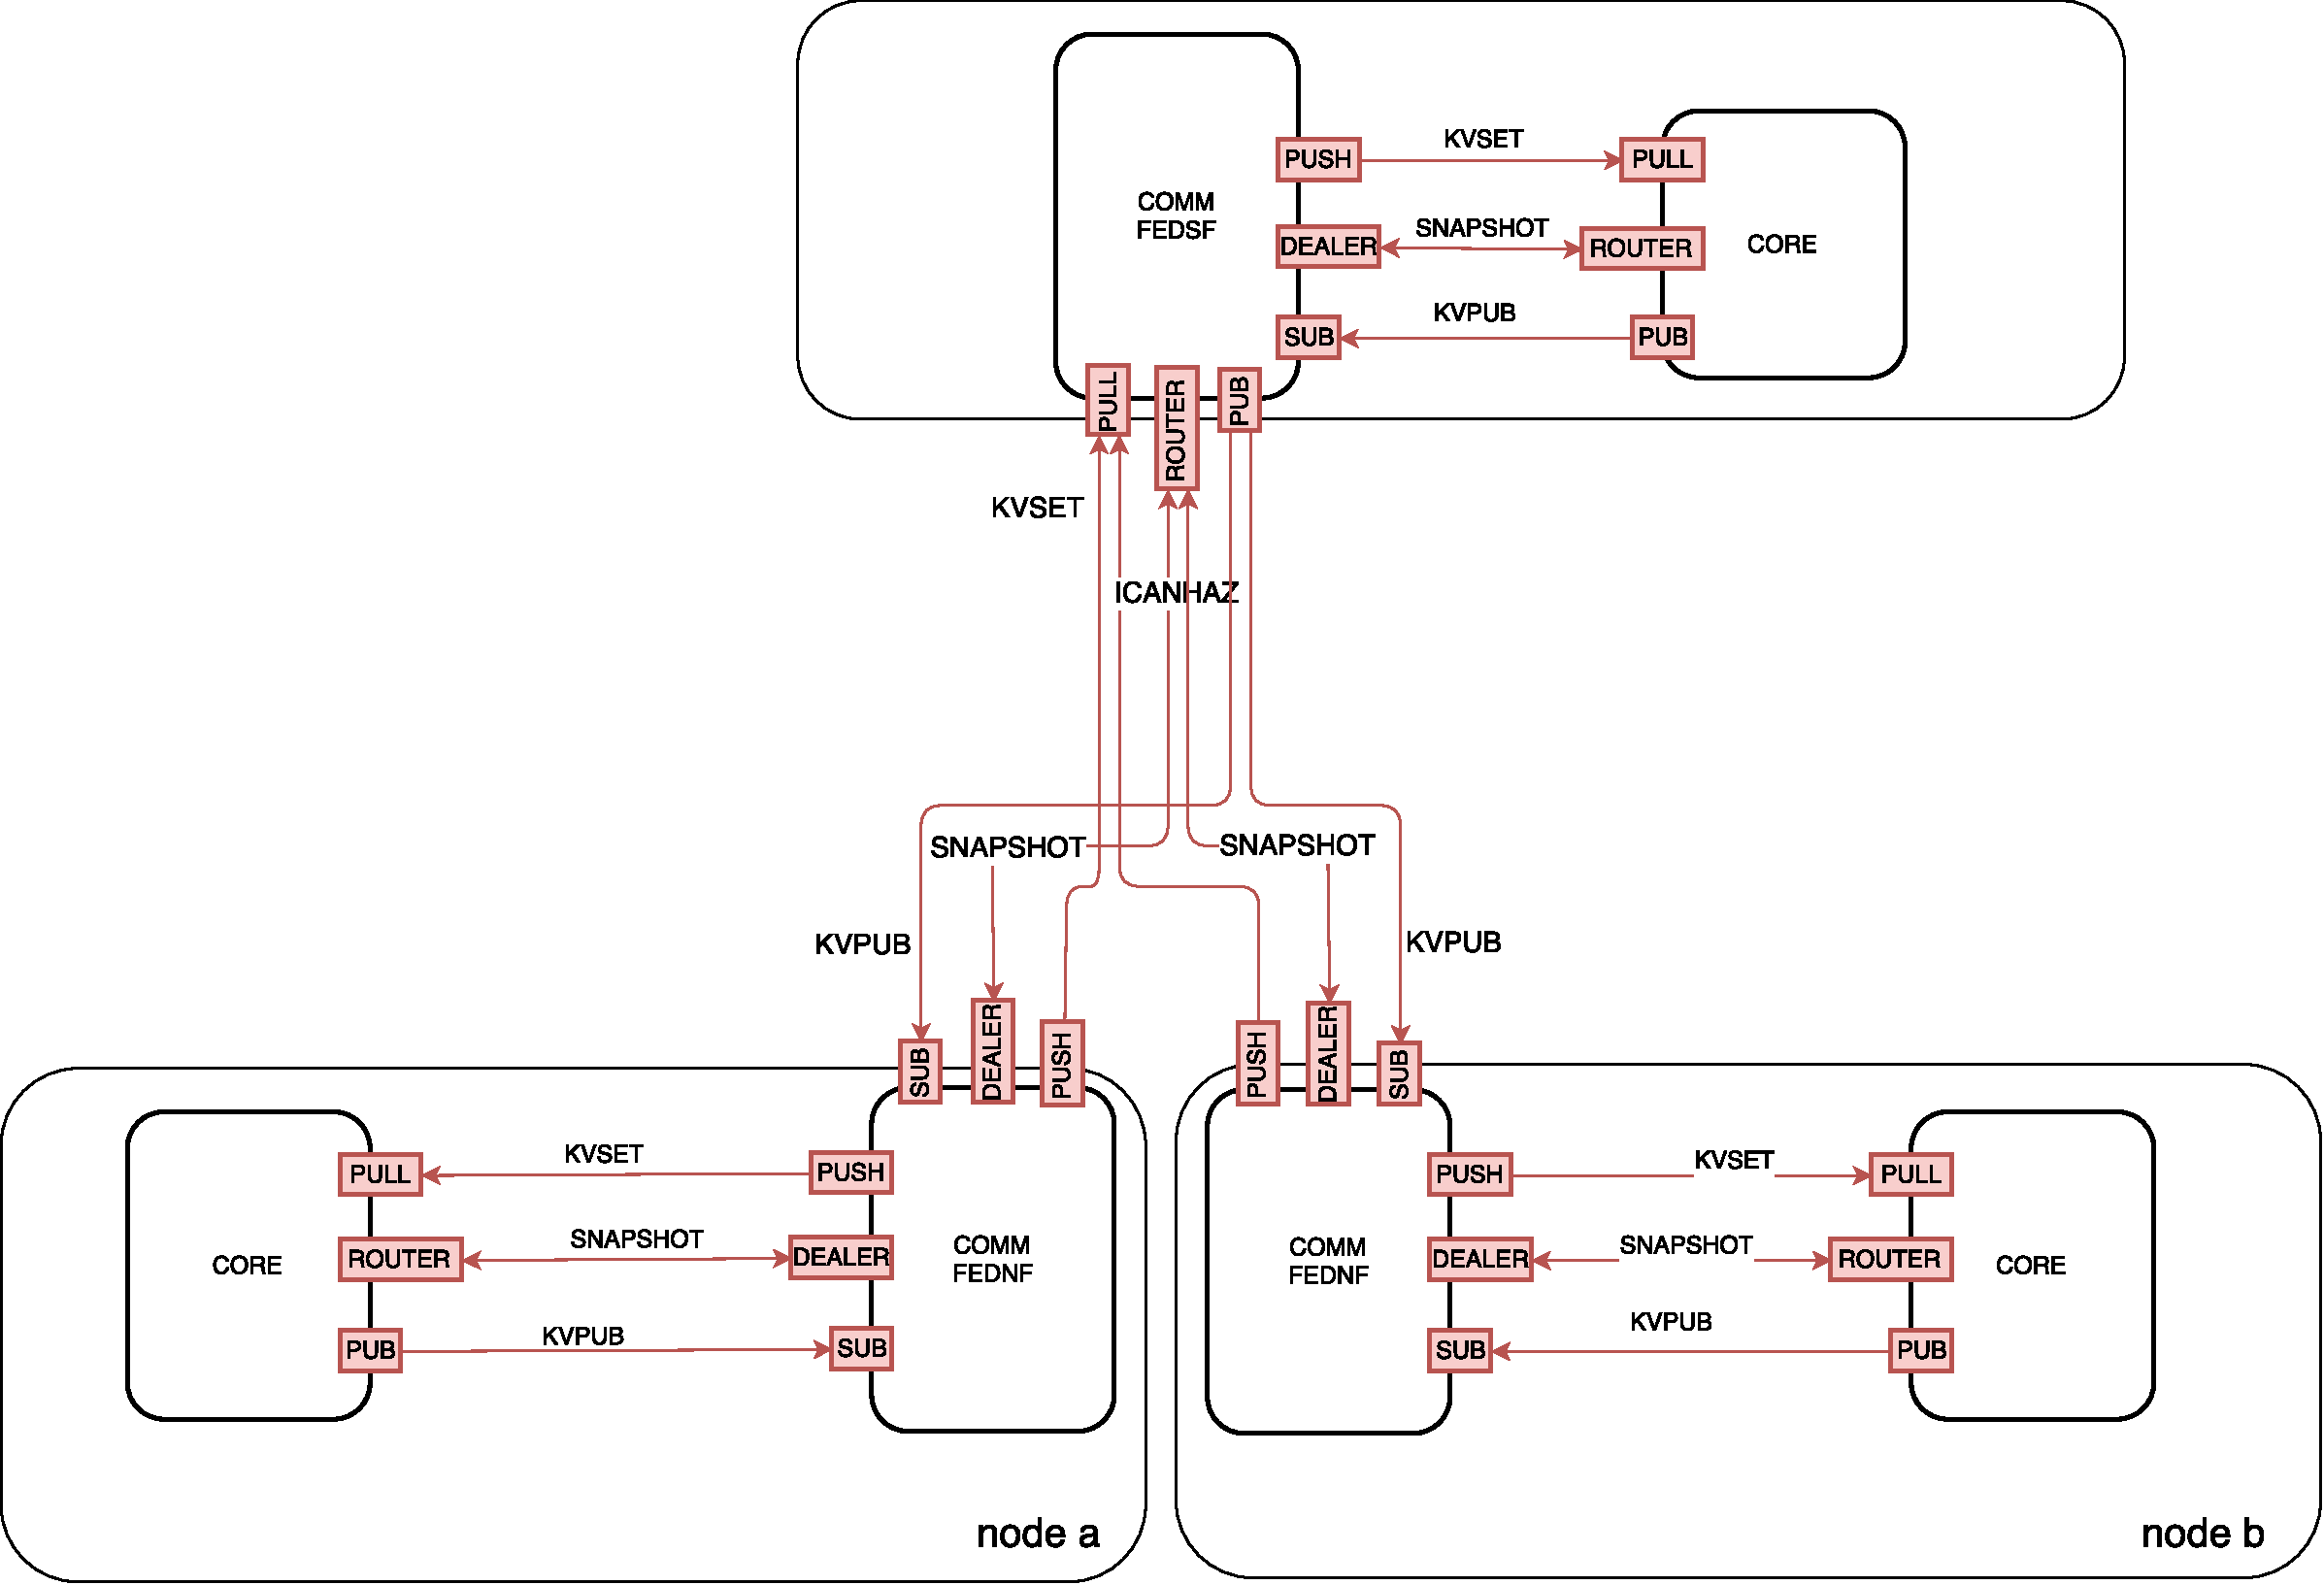
\includegraphics[width=\textwidth]{img/federation_protocol.pdf}
	\caption{Federation between a supernode and two subnodes}
	\label{fig:federation}
\end{figure}

\subsubsection{Fallacies of distributed computing}
At this place, it is worth noting the common fallacies encountered in
distributed computing, as explained on \cite{dcomp:fallacies}.

\subsection{DIM synchronization}
The following is a list of things that are missing before the requirements can be fulfilled:
\begin{itemize}
\item it has to work across several nodes
\item it has to be able to handle HA supernodes, which affects DIM synchronization and message routing
\end{itemize}

There are multiple choices when it comes to what exactly of the DIM should be synchronized:

\begin{description}
	\item [Variant 1. Sync self-subtree only] \hfill\\
	Always sync on subtree only, which means a node only knows the DIM part of
	itself. The big disadvantage is that it won't have a copy of the rest of the
	DIM, which can be useful to inspect variables on neighboring nodes, especially
	when they're unreachable.

	\item [Variant 2. Sync complete tree] \hfill\\
	Always sync on complete tree, which means getting the snapshot from the
	supernode and merge the own subtree into it, replacing whatever subtree is
	already there. This works because of the autonomy requirement for nodes and
	their subnodes. This variant is very easy to implement at first.

	\item [Variant 3. Either sync on subtree or complete tree] \hfill\\
	Make it configurable: Either sync on subtree or on complete tree. The
	toplogy DSL would allow to specify this property for each node. This is
	the best of both worlds, but more effort.
\end{description}

Variant 2 will be the first step. Variant 3 will be the second step, if at all.

Since COMM actors are used to communicate with things outside of a node, new COMM
actors will have to be introduced: One kind that is south-facing to communicate
with subnodes, and another one that is north-facing for communication with
supernodes. They will be named COMM FEDNF and COMM FEDSF. % TODO explain meaning and benefits

Their responsibility is the inter-node synchronization of the DIM, similarly to
what's happening in the existing CSP within a single node.

To send KVSET updates from one actor to the CORE actor, PUSH-PULL sockets are
used. However, similar to the \gls{CHP} described in the \gls{zguide}, this
mechanism here needs to be able to handle replication to one or two (in case of
HA) supernodes. That means using PUB-SUB messaging for is more
appropriate, so all direct supernodes hear the updates.

\subsubsection{CAP theorem}
The CAP theorem \cite{wp:cap} states that it is impossible for a distributed
computer system to simultaneously provide consistency, availability, and
network partition tolerance. In the face of a network partition, one has to
chose between availability and consistency. Because subsystems of a Roadster
federation must be autonomous, availability is chosen.

Eventual consistency is guaranteed by restricting write access to the owning
node, and recovering from a network partition when communication is restored is
done by simply reinitiating the DIM synchronization process.

\subsection{Node topology definition}
The federation topology has to be defined somewhere. This can be done using a
\gls{DSL} and then put into a static file (e.g. \sh{topology_conf.rb}) shared
on all nodes of a Roadster federation. Each actor could then read the file at
startup, just like it's done for other configuration pieces of a Roadster node.
\autoref{lst:dsl:topo:no-ha} shows how such a configuration snippet might look.

To let the actors of a node know which node they belong to, an additoinal line
has to be added to the specific configuration file (\sh{conf.rb}), e.g.
\rb{conf.system_id = "nodes.root"}. Using that information, the topology
created using the DSL can be walked like a tree to find the correct node and
important information like its neighbor nodes.

A HA node pair could be one DIM object which has one name but two IP addresses
(primary and backup, in that order). Direct subnodes can use that information
to connect to the correct supernode during normal operation and also
when the primary node is unavailable. The respective DSL snippet is shown in
\autoref{lst:dsl:topo:with-ha}.

Not every node in a federation has the same role: Some are only connected with other
nodes, some directly communicate with field devices. To define different node roles, a
syntax as shown in \autoref{lst:dsl:topo:with-roles} is possible.

\begin{lstlisting}[style=customruby,caption={Federation DSL example without HA}, label={lst:dsl:topo:no-ha}]
# * basic method to add a node: #add_node(ID, south_facing_bind_endpoint)
# * it takes a block for defining subnodes

conf.nodes do |map|
  map.add_node("root", "tcp://10.0.0.1:5000") do |map|
    map.add_node("subnode_a", "tcp://10.0.0.10:5000")
    map.add_node("subnode_b", "tcp://10.0.0.11:5000")
  end
end

# subnode_a can infer its endpoints from its position in the tree:
conf.system_id = "nodes.root.subnode_a"
#=> this node is "subnode_a"
#=> its IP address is 10.0.0.10
#=> north facing COMM actor's bind port is 5001
#=> south facing COMM actor's bind port is 5000
#=> north facing COMM actor will connect to "root" node on "tcp://10.0.0.1:5000"
\end{lstlisting}

\begin{lstlisting}[style=customruby, caption={Fedreation DSL example with HA}, label={lst:dsl:topo:with-ha}]
conf.nodes do |map|
  map.add_ha_pair("root", "tcp://10.0.0.1:5000", "tcp://10.0.0.2:5000") do |map|
    map.add_node("subnode_a", "tcp://10.0.0.10:5000")
    map.add_node("subnode_b", "tcp://10.0.0.11:5000")
  end
end

# subnodeA can infer its endpoints from its position in the tree:
conf.system_id = "nodes.root.subnode_a"
#=> this node is "subnode_a"
#=> its IP address is 10.0.0.10
#=> north facing COMM actor's bind port is 5001
#=> south facing COMM actor's bind port is 5000
#=> north facing COMM actor will connect to "root" HA pair on "tcp://10.0.0.1:5000" OR "tcp://10.0.0.2:5000" (Lazy Pirate algorithm)

# for primary root:
conf.system_id = "nodes.root[primary]"
\end{lstlisting}

% ############
% # within ba-roadster-app's lib/domain/domain.rb file:
% #
\begin{lstlisting}[style=customruby, caption={Federation DSL example with HA and roles}, label={lst:dsl:topo:with-roles}]
# Idea for node topology definition and assigning roles (features/adapters) to
# diffent kinds of nodes.

module Roadster
  module Domain::Model

    build do
      nodes do
        node "root" do # or maybe ha_node or bstar_node
          endpoint "tcp://10.0.0.1:5000", "tcp://10.0.0.2:5000"
          label 'BA Roadster App'
          desc  'Sample application for experimenting and developing the new features within the scope of the Bacherlor Thesis of Patrik Wenger and Manuel Schuler at HSR.'

          load_conf ::Conf::AccessControl
          load_conf ::Conf::Objects
          load_conf ::Conf::Navigation

          node "subnode_a" do
            endpoint "tcp://10.0.0.1:5000"
            load_conf ::Conf::Adapters
            # load_conf ...
          end
        end
    end

  end # Domain::Model
end # Roadster
\end{lstlisting}


\subsection{Message routing}
Messages need to be sent from an actor on one node to an actor on another node.
The best place to put this logic is the CORE actor which already does this for
messages exchanged within a node. It needs to be extended to know about nodes
and their actors, not only actors on the current node. Then messages can be
passed around hop-by-hop.

In case a message is sent in \emph{Dialog} mode, this implicates Russian doll
routing: At every hop, a new dialog is started which expects an immediate
response, which will subsequently be passed back and complete the open dialogs.

\subsubsection{Example}
When a user of the root node's web UI wants to change a value on a field device
connected to the root node's subordinate node, a command is sent from the
browser to the web UI's COMM actor. From there it's sent via the CORE actor out
on the FEDSF actor to the subordinate node. There it's routed
via the CORE actor to the correct COMM actor, where the command can actually be
executed on the field device.

%----------------------------------------------------------------------------
\section{High availability}\label{sec:approach:ha}
% TODO: HA node => HA peer, backup node => backup peer (??), active peer, passive peer?
If Roadster is going to be run in a federation, measures need to be taken to
mitigate the risk of failure, since many nodes are more likely to fail than a
single node (unless they add redundancy). Availability shall be ensured by
adding redundancy on certain levels of the node hierarchy (e.g. at the bottom
of the topology, right above the PLC, or at the root level), in the form of a
fully functional backup node in addition to the primary one.

Run together in a hot-standby cluster, the passive node's responsibility is to
take over in case the active one goes down.

\subsection{Defining reliability}
When speaking about reliability, it's worth listing the failures we want to be % FIXME
able to handle. According to the requirements, these are exactly:

\begin{description}
	\item [Hardware or software failure on the primary node:]
		This could be one of the actors crashing, the whole OS
		crashing, or a fatal disk failure, irrecoverable memory error,
		or even just someone accidentally pulling the power plug.
		% TODO: more detailed

	\item [Network failure]
		This only includes the failure of the link connecting a HA node
		to the rest of the federation.  Interestingly, this limitation applies to both
		single level and multi level HA.
		% TODO: more detailed
\end{description}

Failures that won't be covered include:
\begin{description}
	\item [Failure of the link between a subnode and one of its supernodes:]

		This can't be handled since the two HA peers would have to
		continually share the number of subnodes connected to them, and
		based on that, make a decision on which one should be active or
		passive. Since the link between them could fail as well, this
		decision can't be done reliably, which could lead to the
		dreaded split brain syndrome.
		% TODO: this protocol extension should be possible, communicate
		% number of fully synchronized clients, if it stays 0 for 3
		% cycles & ICANHAZ requests are coming, backup shall take over


	\item [Failure of the link between a HA peer and the field device]
		The \gls{bstar} algorithm won't initiate a failover since the
		active is still alive and is able to tell the passive node so.
		The missing life signs via the field device could cause an alarm, but no
		failover, since they're only half of the conditions that have
		to be met for a failover.
		% TODO: more detailed
\end{description}

The \gls{zguide} describes a very simple mechanism to achieve this kind of high
availability with exactly two redundant nodes: The \gls{bstar}. It
provides a set of clients a highly available service by running two server
nodes in a hot-standby setup. It is simple and thus very robust, avoids the
split-brain syndrome, and is fairly easy to implement, even as reusable
code. The implementation could be contained within a new kind of COMM actor
called BSTAR. This makes sense since it talks to the outside world.

% TODO maybe we need to extend binary star to handle other kinds of network failures?

\subsection{Binary Star in a nutshell}
Two HA peers are started either as primary or as backup. After an initial
handshake, the primary one becomes active, the backup node becomes passive. The
two continually exchange heartbeats. Clients always connect to the primary's endpoint first.

The passive node takes over when the following two conditions are met:

\begin{enumerate}
\item no life signs from the active node
\item connection requests from clients
\end{enumerate}

The second condition is to prevent the split-brain syndrome and thus can be
thought of as an external vote for the node to actually initiate the failover.
This works because clients will always try to connect to the primary node's
endpoint first, then move on to the backup node's endpoint. This algorithm is
explained in \cite[Chapter 4 - Reliable Request-Reply Patterns, Client-Side
Reliability (Lazy Pirate Pattern)]{zmq:zguide}.

\subsection{Failover}
In case the currently active peer goes down, the two conditions will be met.
This means that the passive node starts accepting snapshot requests (ICANHAZ
messages) and updates the DIM, so every other node will know about the new,
active node. This is needed for the message routing to work.

% TODO: move down?
It's important to mention that a dedicated, direct link from one HA node to its
peer actually worsens high availability. In case the non-dedicated link from
the primary HA node goes down, meaning the HA node is effectively offline and
unavailable for subnodes, the failover won't happen since heartbeats are still
exchanged with the HA peer over the dedicated link.

% TODO No client => no failover

\subsubsection{Alarm generation}
When a failover happens, it makes sense to create a \rb{Case} (alarm) in the
DIM, so the outage is visible to operational personnel in one of the web UIs.
The same applies to the case where the passive node goes down, although it
doesn't have an immediate effect on availability.  This is so the operational
personnel can act upon the alarm and e.g. initiate field forces to inspect the
failed node and repair it.

Once repaired, it's restarted with the exact same configuration --- either primary
or backup. Since there's already an active node (either the primary one,
or the backup one), the newly repaired node will become the new passive node.

\subsubsection{Failover from backup to primary node}
Once failed over, the newly actve backup node stays active. It does so until it
fails itself or is manually stopped. It never automatically switches back to
make the primary node the new active one without a failure. This is key. If a
node becomes unreachable, the failover happens automatically, but anything else will
require human interaction.

Subsequently, when the previously broken, primary node has been repaired, it
rejoins the \gls{bstar} cluster as the passive node. At that point, the backup
node can be killed if need be, and the primary node will take over again.  This
works because the \gls{bstar} operates symmetrically after a successful
handshake during initialization.

\subsection{Side benefit: Rolling upgrades}
% TODO useful for upgrades (maybe in Discussion)

\subsection{A note on dedicated links}
The \gls{zguide} mentions that a dedicated link between the two HA peers
(traditionally done with a crossover cable) is the best solution to prevent the
split-brain syndrome. This is true. But in some cases, it could also prevent a
failover from happening.

Imagine the currently active peer's other network equipment fails, i.e. its NIC
connected to the switch fails, or its switch port fails, then it's unreachable
to the rest of the federation. In that case, a failover would be wanted. But it
can't happen, since heartbeats are still exchanged with the passive node over
the dedicated link. So it's a trade-off between risking the split-brain
syndrome and not being able to perform a failover.

\subsubsection{Extending \gls{bstar}}
Of course the \gls{bstar} mechanism could be extended to
communicate the number of fully connected clients. That way, a passive node
could recognize the situation correctly, since it will get requests from
clients which are trying to fallback to it since the active peer is
unreachable. Knowing its active peer has zero connected clients, it could
actually promote itself to the new active peer.

For this to work, a way of counting fully connected (not just requesting)
clients has to be introduced. Since \zmq abstracts connection handling
completely away, this needs to be done using heartbeats, i.e. from the clients
that are currently fully connected (i.e. registered to receive DIM updates).
This number, or list of clients, could be communicated privately just between
the two HA peers, along with the heartbeats, or it could be published via the
DIM.

Another thing that's needed is a HA peer's ability to step down from being the
active node as soon as its peer promotes itself to the newly active peer. In
the standard \gls{bstar} mechanism, this would be recognized as the split-brain
syndrome and handled fatally.


\subsubsection{Dangerous corner case}
% TODO Backup node active, dedicated link goes down, and there are new/reconnecting clients}
% TODO this will lead to split-brain syndrome (maybe in Discussion)
% TODO in general: dedicated link for HA pair communication is dangerous!

\subsection{Single level}
This is different from what's described in the \gls{zguide} because the concept of
client requests is missing here (field devices don't request anything from Roadster nodes).  What can be
done instead is periodically sending life signs from one node to the other
through the field device by updating some designated memory block. This can actually be
done by both the active and the passive node, which reduces code complexity.

The passive node will check the active node's life signs periodically as well.
In case the life signs cease, it can give its vote to the COMM BSTAR actor.
This would satisfy the second condition of the \gls{bstar} for a
failover to take place. The first condition would be the missing heartbeats
which are normally transmitted through the network link.

TODO new actor: COMM BSTARVOTER (or maybe directly into CORE actor)

\begin{figure}[]
	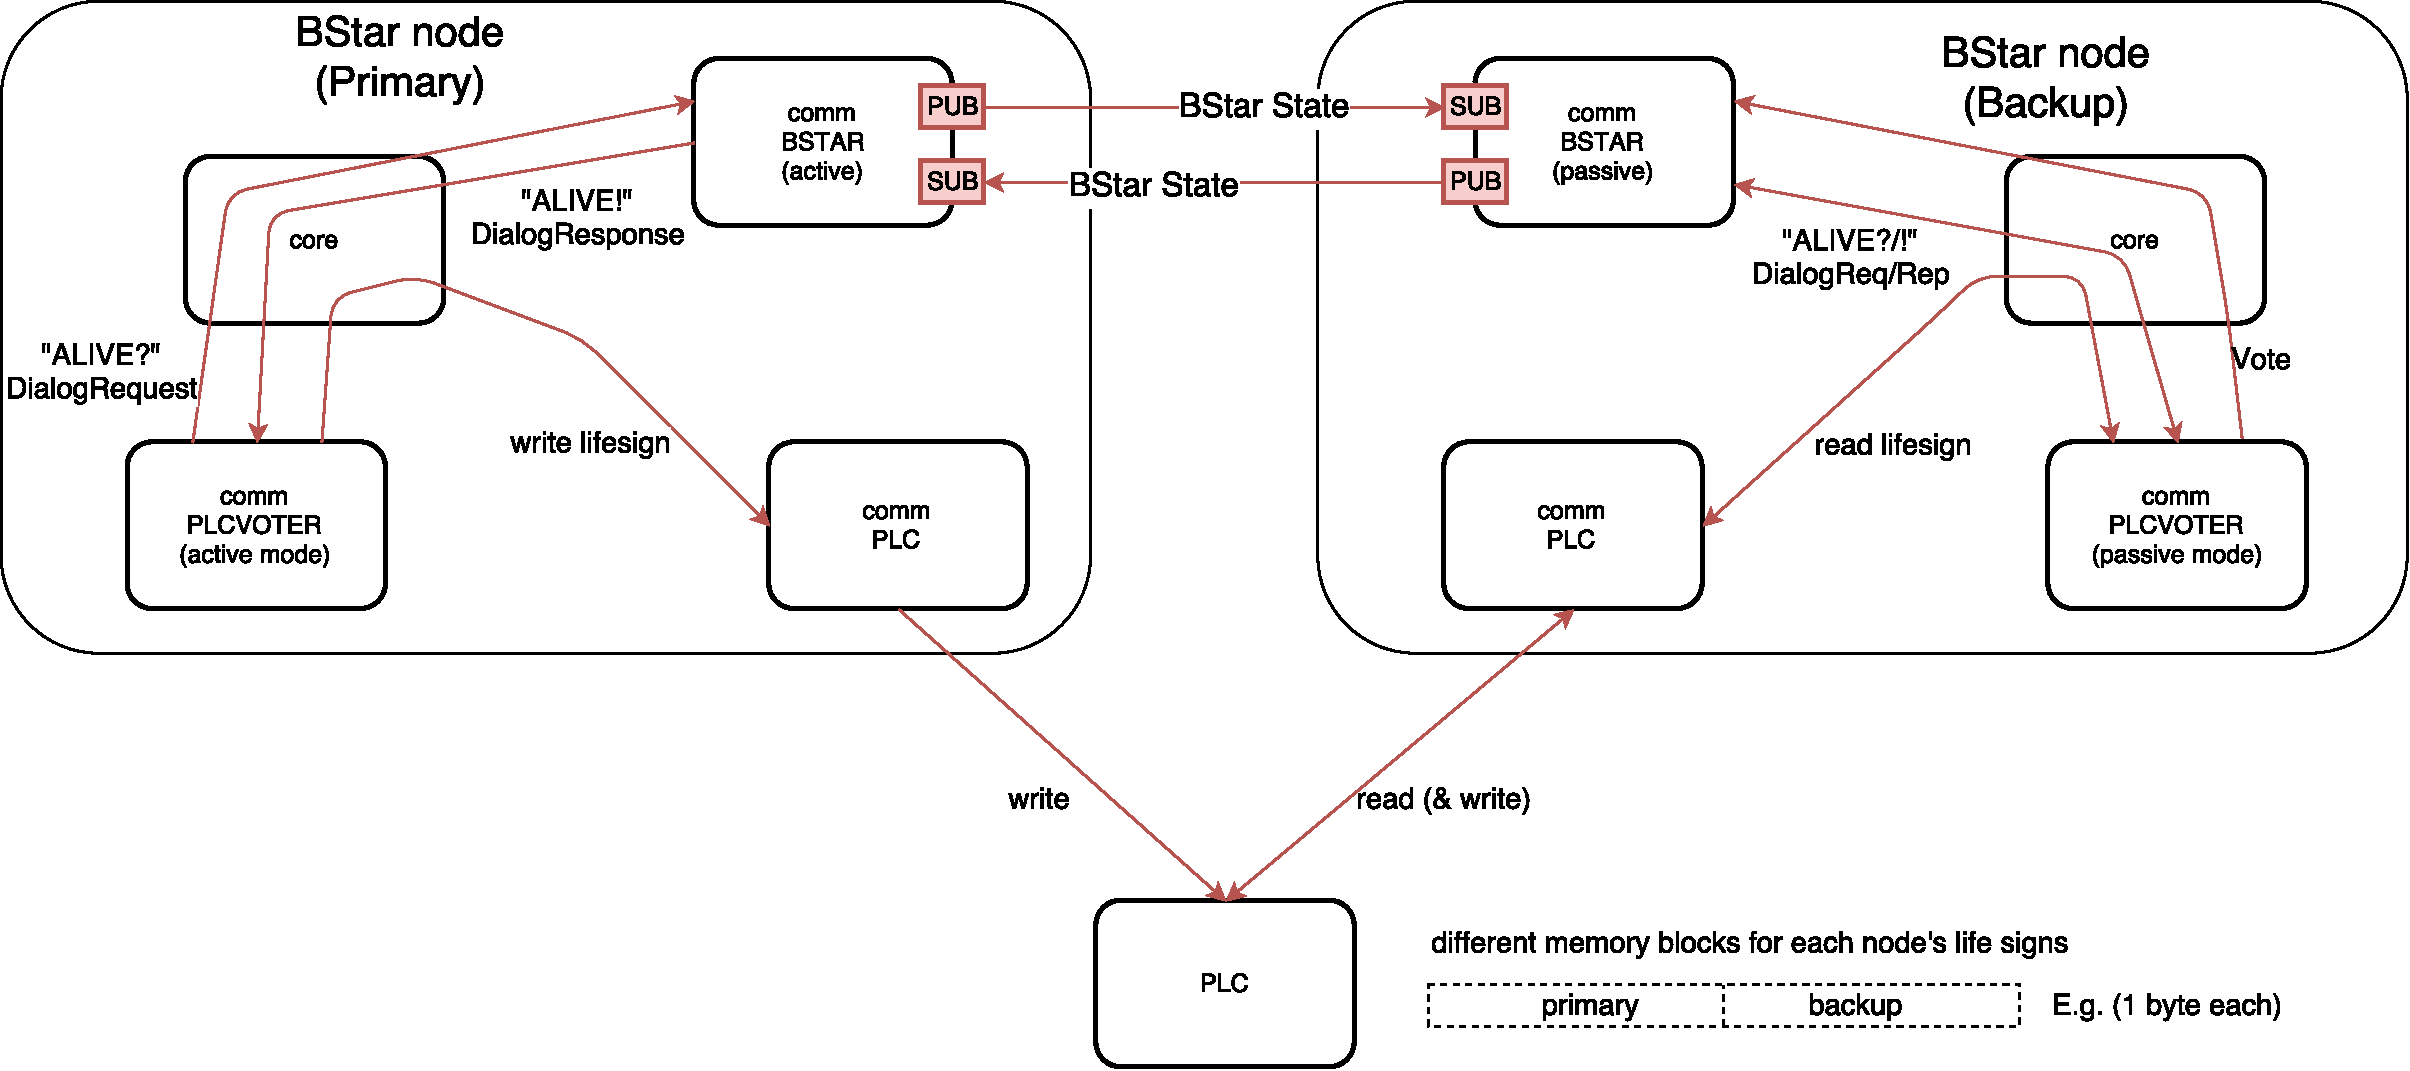
\includegraphics[width=\textwidth]{img/SL-HA_bstar.pdf}
	\caption{Single level HA setup between a HA pair and a field device (PLC)}
	\label{fig:sl-ha}
\end{figure}
% TODO: mention figure in text

\subsubsection{Caveats}
Special attention needs to be paid when it comes to writing these life signs. A
na\"ive developer might implement the COMM BSTARVOTER so it autonomously causes
life signs to be written on the field device. This works as long as the failures only affect
the hardware. But what if a software error happens in the CORE or BSTAR actor?
They'd crash or hang, while the BSTARVOTER happily sends out life signs, which it
obviously shouldn't be doing at that moment.

A better implementation would have the BSTARVOTER poll the BSTAR via the CORE
router whether it's still alive, and only send out a life sign in case it gets
an answer. This way, the BSTAR and the CORE actor are being tested for
responsiveness. We'll call the two messages being sent back and forth "DEAD?"
and "ALIVE!".

\subsubsection{Link failure between Roadster node and field device}
TODO describe why this won't cause a failover and thus can't be handled, as
mentioned above\\

\subsubsection{Supporting different field devices}
TODO: adapter

\subsection{Multi Level}
This kind of \gls{HA} setup is closely related to the \gls{bstar} described
in \cite[Chapter 4 - Reliable Request-Reply Patterns, High-Availability Pair
(Binary Star Pattern)]{zmq:zguide}. This means that the passive node would
actually receive requests from clients in case the active node fails, which
simplifies the implementation. These requests will count as votes to fulfill
the second condition that has to be met for a failover to be initiated. This is
illustrated in \autoref{fig:ml:ha}.

\begin{figure}[]
	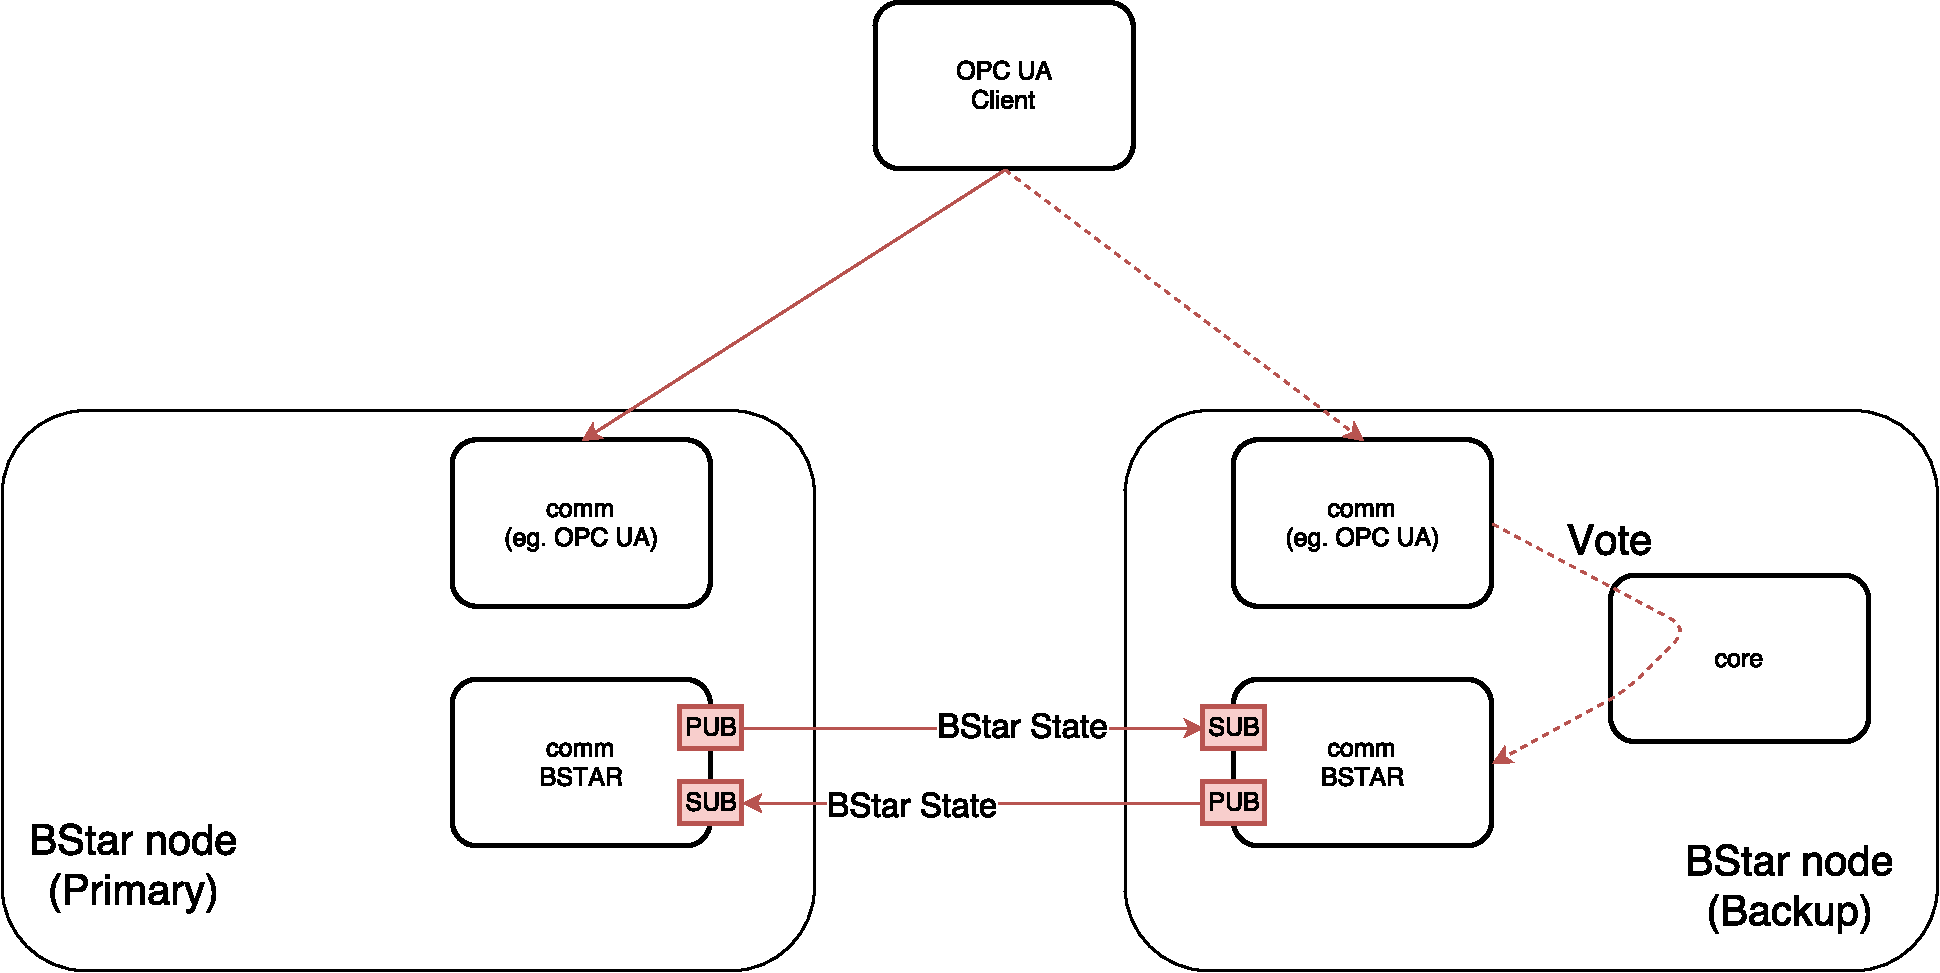
\includegraphics[width=\textwidth]{img/ML-HA_bstar.pdf}
	\caption{Multi level HA setup between a HA pair and a number of client nodes}
	\label{fig:ml:ha}
\end{figure}

%----------------------------------------------------------------------------
\section{Persistence synchronization}\label{sec:approach:psync}
The persisted data and updates to it, handled by the STORAGE actor, need to
bubble up and collected in the root node.

\subsection{Aspects}
There are multiple aspects involved in persistence synchronization:

\begin{description}
	\item [Initial synchronization:]
		How does one get the initial delta of updates since the last
		synchronization?

	\item [Continuous synchronization:]
		Further updates, one-by-one. This is only needed in
		case the solution aims for instantaneous synchronization.

	\item [HA peer sync:]
		How is the passive HA peer updated?
		This not only matters when the supernode is a HA pair (multi
		level), but also when it's at the bottom of the node hieararchy
		(single level).

		% TODO
		\large\color{red} What about that last case? We need to synchronize
		east-west. Something similar as with Binary Star, where updates
		go into a \emph{pending} queue on the passive node until
		confirmed by the active node?
\end{description}

\subsection{Variants}
There are multiple variants to achieve the needed functionality.
% NOTE: Client seems to favor polling.

\subsubsection{Polling only}
The supernode just periodically request persistence
deltas. This would be handled over a DEALER/ROUTER pair of sockets. The nice
thing about this variant is that the subnode only has to do one thing, which is
responding to requests from the supernode(s); it doesn't have to proactively
send any updates after sending the an initial delta.

A big drawback is that the synchronization doesn't happen instantaneously. This
doesn't seem to fit well into the overall Roadster architecture, which is
completely event-driven (no polls or "sleeps").

Another drawback is efficiency. This variant will periodically cause the
subnode's database to be searched for all keys. Depending on the size of the
database and the efficiency of searching through keys, this could be a lot of
wasted resources or even cause bottle necks when interacting with the STOR
actor.

In case the supernode is a HA pair, this variant would generate duplicated
traffic. To avoid this, another pair of sockets has to be introduced to
synchronize persistence between a HA pair. This also means designing another
protocol, and more moving parts overall.

% TODO: SL-HA

Overall, this variant is very simple, but doesn't offer some features we'd
normally expect from a framework like Roadster. The fruits are hanging low;
achieving instantaneous synchronization and better efficiency is easy.

\subsubsection{PUSH-PULL}
This variant avoids the delays introduced by the polling mechanism of the first variant.

Procedure (for each subnode):
\begin{enumerate}
	\item via a ROUTER/DEALER socket pair:
		\begin{enumerate}
			\item supernode tells subnode its most recent timestamp in an ICANHAZ request
			\item subnode sends delta
			\item supernode receives and processes the complete delta
		\end{enumerate}
	\item subnode sends updates to supernode via PUSH-PULL
	\item during low-traffic times, we can send HUGZ as heartbeats
\end{enumerate}

This seems nice at first, but the PUSH socket's send buffer will fill up when the
connection is interrupted.  This isn't bad in and of itself, because when it's
full (and writes start to block), we can just destroy the socket and
reinitialize and start syncing anew (from ICANHAZ) after a certain timeout.
But the problem is that, in case the delta is large, it will inevitably fill
the PUSH socket's send buffer, temporarily reaching its high water mark, which
is part of its normal operation.

So we'd have to introduce logic to recognize whether the PUSH
socket is just temporarily full (e.g. during delta transmission), or
permanently full (e.g. the supernode or the link to it is down).

% TODO: SL-HA

Another disadvantage is that there needs to be another channel to synchronize
persistence updates to the other HA peer, if there is one. This means another
pair of sockets, another protocol to be designed, and more moving parts
overall.

\subsubsection{PUB/SUB}
This is similar to \gls{CSP}/\gls{CHP}. It's not 100\% reliable, but even with unstable
links, no data loss will occur if the client (the supernode) is able to reconnect within a
specific amount of time. \zmq's default for that amount is 10 seconds. As the
requirements specify, 100\% consistency is not mandatory for the persistent
data.

A possible drawback is that the traffic is duplicated in case the supernode
is a HA pair. However, there are numerous opportunities to mitigate this.

Procedure (for each subnode):
\begin{enumerate}
	\item supernode subscribes to updates from subnode
	\item via a ROUTER/DEALER socket pair:
		\begin{enumerate}
			\item supernode tells subnode its most recent timestamp in an ICANHAZ request
			\item subnode sends delta
			\item supernode receives and processes the complete delta
		\end{enumerate}
	\item supernode starts reading updates, possibly skipping the first few (based on timestamp)
\end{enumerate}

% TODO: SL-HA

\subsection{Chosen Variant}
We'll most likely go with the PUB-SUB variant, since it's simple and is similar to
what's used for the new \gls{CSP} in conjunction with multi-node \gls{HA}. It provides the best
opportunities to improve efficiency later on.

Its possible performance issues can be ignored right now, as trying to fix them
is arguably considered premature optimization. If this turns out to be an issue
in a productive deployment, like over a cellular network link, a future version
can switch to multicast. \zmq supports PGM, which is a reliable multicast
protocol. (Pragmatic General Multicast, standardized, directly on top of IP,
requires access to raw sockets and thus may require additional privileges) and
EPGM (Encapsulated Pragmatic General Multicast, encapsulated in a series of UDP
datagrams, doesn't require additional privileges, useful in a \zmq-only setup).

If its reliablity turn out to be an issue, one the socket option
\sh{ZMQ_RECOVERY_IVL} can be increased from 10 seconds to, say, 60 seconds, which
gives an unstable link more time to recover before any data loss happens.

TODO: describe reasonable default setting, in case we change ZMQ's default.


\section{Security}\label{sec:approach:security}
The simplest variant of enabling transport security, as described in
\autoref{sec:zmq:security} is to allow any client to connect. The clients still
have to be in possession of the server side's public key. Depending on the
number of levels in the node hierarchy, that or those public keys can be
distributed conveniently and safely through the node topology configuration
file. Public keys are only 40 characters long in \gls{Z85} notation.

Only the server's public key has to be distributed on the respective client nodes
securely and in advance, which might be considered inconvenient, depending on
the number of nodes and distribution method.

% amplification attacks, message size, ...

% TODO: variant with central ZAP server: bad, because of lost autonomy

\subsection{Key generation and distribution procedure}
The following procedure can be followed to generate the required keys in
advance and make them available through the shared configuration file:

\begin{enumerate}
	\item for all nodes that will have sockets that will act as CURVE servers (i.e. all non-leaf nodes)
	\begin{enumerate}
		\item generate key pair and save it on the respective node
		\item for each direct subnode
		\begin{enumerate}
			\item put a copy of the public key (in Z85 notion) into that node's block within the shared topology configuration file
		\end{enumerate}
	\end{enumerate}
\end{enumerate}

This procedure could be implemented as a script that generates the keys and
distributes them via \gls{SSH}.

\subsubsection{Client authentication}
In case client authentication is actually desired, the clients' keys also have
to be generated in advance, and the public key files for each subnode of a
supernode in question have to be stored into a directory. That directory can
then be specified to the \rb{CZTop::Authenticator} actor.

\subsection{In code}
\autoref{lst:auth:any} shows how to start an authentication handler which
allows any client to connect, effectively only allowing authenticated
encryption, but not a true client authentication. What it actually does is
start an in-process thread to which can be communicated via a PAIR-PAIR socket
pair (it's a CZMQ actor\footnote{CZMQ provides a very simple actor framework
based on threads communicating over \zmq sockets,
\url{http://api.zeromq.org/czmq3-0:zactor}}). The thread calls a
function\footnote{The function is \cpp{zauth()} and is described along
with its capabilities here: \url{http://api.zeromq.org/czmq3-0:zauth}} (passed
as a function pointer at actor creation) provided by CZMQ, which understands
the \gls{ZAP}, different security mechanisms (NULL, PLAIN, and CURVE) and is
capable of reading client public keys from a directory on the file system and
even listens to changes in that directory.

\begin{lstlisting}[style=customruby,caption={Starting an authentication handler that allows any clients}, label={lst:auth:any}]
##
# on the supernode:

authenticator = CZTop::Authenticator.new
authenticator.verbose!
authenticator.curve # use CURVE mechanism, but allow any

##
# start the server sockets
# ...
server_cert = CZTop::Certificate.load("/path/to/private_key")
pub = CZTop::Socket::PUB.new
pub.CURVE_server!(server_cert)
pub.bind("tcp://*:1234")

#############################################################################

##
# on the subnode:

server_cert = CZTop::Certificate.load("/path/to/server_public_key")
client_cert = begin
  CZTop::Certificate.load("/path/to/client_private_key")
rescue Errno::ENOENT # file doesn't exist
  CZTop::Certificate.new.save("/path/to/client_private_key") # generate
  retry
end

sub = CZTop::Socket::SUB.new
sub.CURVE_client!(client_cert, server_cert)
sub.bind("tcp://*:1234")
\end{lstlisting}

\section{OPC UA Interface: High availability}\label{sec:approach:opc-ua}
The OPC UA standard seems pretty complicated. And given that the requirement
isn't concrete yet, no possible solution has been worked out yet.

In case it's non-transparent server redundancy, \cite[6.4.2.4 Non-transparent
Redundancy, p.~96]{opc-ua:behavior:server-redundancy} describes the exact
behavior.

% TODO study standard
% TODO use Andy's gem (it "should be a simple thing")

% vim: ft=tex
\chapter{Results}
TODO what are the results (without discussing them)\\
TODO these is probably the "Implementation"\\

\section{Port}\label{sec:res:port}
TODO explain results here\\


\section{Cluster}\label{sec:res:cluster}
TODO explain results here\\


\section{High Availability}\label{sec:res:ha}
TODO explain results here\\

\subsection*{Single Level HA}\label{sec:res:sl-ha}
TODO explain results here\\

\subsection*{Multi Level HA}\label{sec:res:ml-ha}
TODO explain results here\\

\section{Persistence Synchronization}\label{sec:res:psync}
TODO explain results here\\

\section{Security}\label{sec:res:security}
TODO explain results here\\

\section{OPC UA Interface: High Availability}\label{sec:res:opc-ua}
TODO explain results here\\

% vim: ft=tex
\chapter{Discussion}
% TODO something like a SWOT analysis here (strengths, weaknesses, opportunities, threats)
% TODO general advice: be concise, brief, and specific
% TODO: modifications to the same DIM objects from different actors at the same time => one update will be lost, but consistency is still guaranteed

% TODO: maintainability (SOLID principles, composition over inheritance)
% TODO: additional goal: security of SCADA applications
% TODO: additional personal goal: how fallacies of distributed computing are handled


% performance improvements
%   * circumvent scrypt in test suite
%   * avoid regex, use bare strings if possible (s[s.rindex('@')+1..-1]
%   * test suite with profiling activated
% * future feature: DIM visibility: :federation, :node, :actor
%   - useful for supernode's last_seen (:node), currently an ivar in engine
%   - current choice of HA supernode's endpoints (:node)
% * when closing cases, the flag "all_cases" could fuck up
%   - especially with multiple nodes
%   - with single node: race condition, reply could contain a case (now closed) that was not shown in the UI => what to do?
%   - proposal: remove flag, always just send array of case IDs
% * maybe: model updates are sent to UI before authentication (TODO: tell Manu)
% * ideas:
%   - crystal for performance
%   - msgpack for safety, show benchmarks
%   - broadcast messages, signing, domain model level signature so snapshots can be relayed
% * IDEA for DEPLOYMENT
%   * 1 git repo per deployment
%   * keygen phase: on each node, gen key and git commit in fedrb file
%   * `roadster keygen FILE`
% * analysis of encrypted traffic is still possible (see CURVE zmq)
% * cleartext ZMTP commands
% * talk about factories (MsgPack packer/unpacker) and hook methods, template method

% TODO sign config file: => trash

\section{Value Added}
% TODO what's better than before

\section{Limitations}
% TODO identify potential limitations and weaknesses of the product
% limitation: to followed HA nodes in a layer aren't possible (middle layer with HA and supernode with HA) the problem is the diagonal approach (upstream)
% solution: share data over the bstar sockets and don't use the upstream with the diagonal approach
% weakness: message packages can be identified and if someone would capture the traffic it would be possible to assign the payload to the right
% message type. => solution: filled it with padding...
%  
Limitations imposed by the design and implementation of the new features are
discussed here.

\subsection{Federation}
\subsubsection{DIM replication}
Eventual consistency is guaranteed even in situations where multiple actors
modify the same DIM objects at roughly the same time. However, some updates
might get lost. In those cases, the last writer wins.


Subtree synchronization has not been implemented, as deemed as not necessary at
this moment. Replication performance is by far sufficient, with messages being
sent and received within 1 -- 3 milliseconds, and the space requirements of a
complete DIM was observed to be very small so far, being just a small number of
plain Ruby objects.

\subsubsection{Message routing}
% TODO: would have been easier if CORE had inter-node sockets itself, but: 
% seperation of concern would be injured and the core would be come a big fat monolythic class

\subsection{HA}
A HA cluster has to be complete (both nodes running) during initialization.
Otherwise, only primary node can start to serve requests; the backup node will not
do this.

% TODO refactoring ideas: HANode < Node
%  => root object in config

\subsection{Persistence replication}
Message traffic towards root node sums up because of persistence
replication. This should not be a problem because of \zmq's brilliant
message batching, so the real limit only given by the inter-node network links.

\section{Business Benefits}
Using the new federation capability, Roadster can be deployed in larger
environments, possibly replacing higher-level systems described in
\autoref{sec:scope:sys-integration}.

\section{Ideas for Improvement}
\subsection{High availability}
% TODO: opportunity: Only go active with enough votes

\subsubsection{Thoughtful heartbeating}\label{sec:discussion:imp:ha:hb}
The BSTAR actor currently happily exchanges heartbeats with the BSTAR actor
running on the other HA peer, even in case all actors but CORE are dead. The
CORE actor's health is periodically checked using the PING/PONG mechanism as
described in \autoref{sec:approach:ha:hb}.

In a subsequent version of Roadster, the CORE actor could relay those PING
requests to the other actors and only respond with a PONG in case the other
actors all have responded with PONG. This mechanism would make the node only
signal life signs in case all actors are healthy.

\subsubsection{HA within a node}
Building upon the previous idea, unhealthy actors could be killed and respawned
by the CORE actor.  Microrebooting unhealthy components without an attempt at
any sophisticated recovery would make Roadster belong to the \emph{crash-only} kind of fault-tolerant software.

\subsubsection{Manual failover}\label{sec:discussion:ha:manual-failover}
A manually induced failover could be useful in some cases, e.g. when a
component fails that does not provoke an automatic failover.

Providing a less brutal way of inducing a failover than to turn off the
currently active HA peer could be interesting in a future version.

\subsubsection{Unplanned topologies}
% TODO
HA cluster can't have supernode right now, because upstream's DEALER socket
can't decide which node receives a message sent.
% Solution 1: ROUTER-ROUTER communication between node and subnodes.
% Solution 2: Refactor:
%   - rename Engines::BStar into Engines::Sidestream
%   - publish CSP updates over PUB socket as well (just like from Downstream->Upstream)
%   - add DEALER socket (DEALER-DEALER communication works)
%   - PUSH/PULL socket not needed because passive won't change DIM
%   - primary always binds, backup always connects
%   - => Upstream/Downstream are back to a single responsibility only
%   - => Upstream does not even have to be started on HA nodes
%   - => Downstream only needs to be started with subnodes

\subsection{Miscellaneous}
% TODO check IEEE abstract.. we need a refrence from IEEE as a idea for future features
http://ieeexplore.ieee.org/abstract/document/1541189/ Dynamic distributed computing would allow a Roadster federation to grow without to restart each of then nodes.
http://ieeexplore.ieee.org/stamp/stamp.jsp?arnumber=7190458 When a roadster have to calculate a high amount of data, it could be outsourced to other nodes which have free cpu.
Therefore would be a Data Mining Algorithm a good solution.

Unordered list of ideas:
\begin{itemize}
	\item switch to Moneta for a unified key-value store interface, then eventually away from \gls{tc} to something more modern and maintained, like LMDB (it is super fast and crash-proof)
	\item TIPC: high performance cluster communication protocol, suitable because Roadster nodes are Linux and there are direct links to peers (required for TIPC)
	\item key management in a DB (instead of files), with GUI to accept new clients
	\item dynamic node topology (maybe via DSL-file in Etcd, or DIM-only, or Zookeeper)
	\item other method for data serialization (like MessagePack), would allow adding other programming languages to the cluster
	\item fast compression for messages, like LZ4 or Snappy
	\item SERVER/CLIENT sockets from ZMQ 4.2 for simplified message routing
	\item Ruby \rb{Integer} class instead of \rb{Fixnum}
	\item (use more symbols instead of strings, e.g. to refer to a certain actor)
	\item \sh{ZMQ_RECONNECT_IVL} and \sh{ZMQ_RECONNECT_IVL_MAX} especially for mobile clients
\end{itemize}


% vim: ft=tex
\chapter{Conclusion}
% TODO write conclusion, overall experience and opinion of product\\
% TODO they should teach the actor model in APF, because ...\\

% TODO don't fear the code

% TODO red/green/refactor cycle

% TODO: awesome technologies
% Ruby <3
% RSpec (<3)
% ZMQ <3
% Roadster <3
% layered architecture <3
% NaCl <3
% Crystal <3
% Latex <3
% Gitlab <3
% Python (<3)
% mininet <3
% Docker <3
% MsgPack <3
% lots of time lost with CSP
% CZTop: software design proven, it worked like a charm



\printbibliography
\printglossaries

%-----------------------------------------------------------------------------
\appendix
\part{Appendix}
\chapter{Self Reflection}
TODO how did we perform, completion of goals, accuracy of estimated efforts, efficiency, resourcefulness

\chapter{Task Description}\label{ch:task-desc}
The following five pages are the original task description, signed by Prof. Dr. F. Mehta.
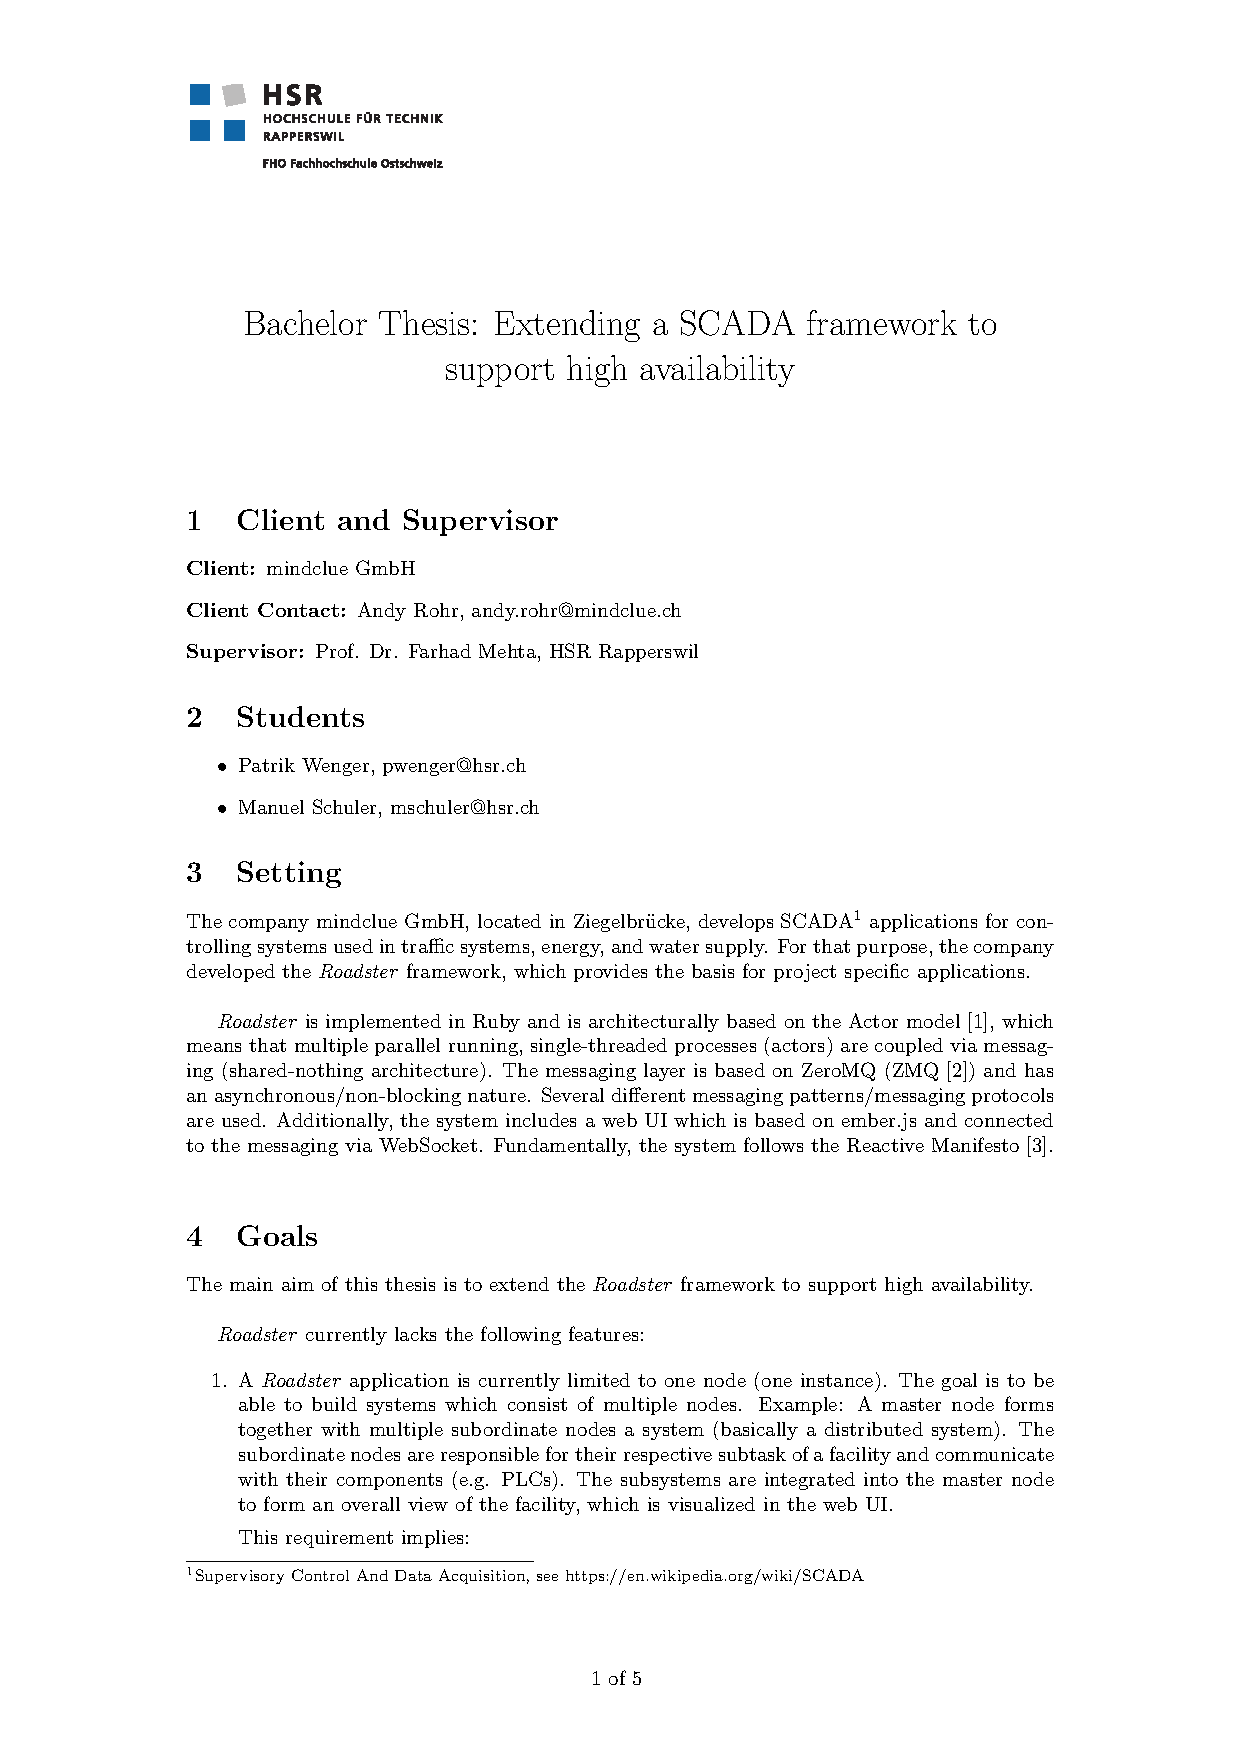
\includepdf[pages={-}]{signed_task_description.pdf}

\chapter{License}
As stated in the task description, all of our code contributions underlie the
ISC license, which is functionally equivalent to the MIT license and the
Simplified BSD license, but uses simpler language. In addition to that, we
hereby explicitly grant mindclue GmbH unrestricted usage of all our code
contributions.

% NOTE: meeting minutes are kept online
% NOTE: time reports are kept online

% vim: ft=tex
\chapter{Project plan}
\section{Software development process}
The \gls{RUP} is used to plan and manage this term project. It’s an iterative,
structured, yet flexible development process which suits this kind of project.
At HSR, it’s taught as part of the Software Engineering courses and is thus a
primary candidate.

Another candidate was Scrum, which we decided against as it’s only feasible
with teams of three to nine developers.

\section{Timetable}
\subsection{Estimated time}\label{sec:projplan:est-time}
The project spans from September \nth{19} until December \nth{23}. We expect a
necessary effort of about 28.5 hours a week which results in a total of
400 hours per group member. See \autoref{tab:timetable}.

\begin{table}[H]
  \centering
  \begin{tabular}{|p{100mm}|p{35mm}|}
    \hline 	\bf Project duration & 14 weeks \\ \hline
	\bf Manpower & 2 \\ \hline
	\bf Effort per person & 28.5 hours per week \\ \hline
	\bf Total estimated time without weighted damage & 720 hours \\ \hline
	\bf Total estimated time including weighted damage & 856 hours \\ \hline
	\bf Project start & September \nth{19} 2016 \\ \hline
	\bf Project end & December \nth{23} 2016 \\ \hline
  \end{tabular} \\
  \caption{Timetable}
  \label{tab:timetable}
\end{table}

The average between best case and worst case is $\frac{720 + 856\,hours}{2} =
788$ hours. Counting in a reserve of 10\% more of additional effort that might be needed to
mitigate materialized risks, this results in $788\,hours + 10\% *
136\,hours\approx 800$ hours of total effort.


\subsection{Time tracking}
All time spent on the bachelor thesis are done on Everhour. Every time record
is associated with a GitHub issue where applicable.
The estimated time is set directly on each GitHub issue using the Everhour pluign.

Everhour allows the export of all time spent on a project, which will be
included as part of the final submission of this bachelor thesis.

\subsection{Quality assurance}


\subsubsection{Software}
To ensure a consistent code quality in the main development branch
(\emph{master}), unit tests and integration test are run before every push of
new changes to the repository on GitHub. Any pending issues found are to be
fixed before the push.


The development of larger -- requiring more than one commit -- features is done
on a specific feature branch.  Upon completion, instead of merging the branch
directly into the main development branch, a pull request is opened on GitHub.
This allows the other student and/or the client to review, discuss, and improve
the changes. The final merge is to be done by a person other than the one who
opened the pull request.

\subsubsection{Documentation}
Important sections are proof read by the co-student and discussed during the
weekly stand-up meetings.

At the beginning of this bachelor thesis, the professor has been consolidated
for inputs regarding the structure of this document. His advice has been
respected as far as feasible.

Andy Rohr from mindclue GmbH has assisted as another proof reader, especially
for technical correctness regarding the Roadster framework.


\subsection{Meetings}
Meetings are called for by the students on an as-needed basis in consultation
with the professor or the client. Prior to a meeting, the students prepare a meeting
agenda on the wiki of the documentation repository on GitHub.

The meeting agenda for meetings with the professor include the new progress
(incremental), problems, agenda (such as administrative questions), and
short-term goals.

After each meeting, the students follow up by writing down meeting minutes
which include the list of actual participants, decisions made, and pending
tasks.

In addition to the meetings with the client and the professor, the students
hold a weekly standup meeting placed in early/mid-week, which is to be a short
exchange of the current project status, review of the last week, and a
discussion of the next short-term steps.

\subsubsection{Review}
By the end of the bachelor thesis, a total of six meetings (including the
kickoff meeting) have been conducted together with the professor. The meeting
minutes are on \cite[Meetings]{gh:wiki}.

The client mindclue GmbH has been met four times. The first meeting was to
gather the requirements during the first week. The second meeting was necessary
to clarify the requirements and decide upon a more structured format of the
requirements (Cucumber features). The third meeting took place during the
second Elaboration iteration to help with Roadster's codebase in preparation of
the upcoming construction phase. The last meeting was a code review meeting
after the first Construction iteration. Further code reviews were performed
directly on GitHub.

Acute discussions and more lightweight decisions with the client were held on
the particular GitHub issues \cite{gh:issues} directly, as well as the Slack
communication platform.


\section{Risks}
There were nine risks that have been identified by the end of the Inception phase.
The risks have a total damage of 369 hours. The total damage hours multiplied
by the probability of admission result in a total of 137 hours. The weighted damage
hours are included in the project planning.

\subsection{Handling risks}
Due to the nature of the risks, it is only natural they change over the course of a project.
To mitigate this, the risks are checked regularly (in weekly meetings) using \autoref{tab:init-risks}.

Changes to existing risks are possible. This usually means that either the likelihood or
the unweighted damage must be adapted immediately. Moreover, it is possible for a risk to
be completely ruled out, or that a new risk arises. All these points need to be discussed in
the team and tracked accordingly.

\section{Listed risks}
\begin{tabular}[t]{@{}>{\raggedright}p{0.45\textwidth}}
  \textbf{\textit{P = Probability}}
  \begin{enumerate}[topsep=0pt,itemsep=-2pt,leftmargin=13pt]
  \item Rare (10\%)
  \item Unlikely (30\%)
  \item Possible (50\%)
  \item Likely (70\%)
  \item Certain (90\%)
  \end{enumerate}
\end{tabular}
\begin{tabular}[t]{@{}>{\raggedright}p{0.52\textwidth}@{}}
  \textbf{\textit{D = Damage potential  / R = Risk}}
  \begin{enumerate}[topsep=0pt,itemsep=-2pt,leftmargin=13pt]
  \item Insignificant
  \item Negligible
  \item Moderate
  \item Serious
  \item Significant
  \end{enumerate}
\end{tabular}

\autoref{tab:init-risks} lists the initially identified risks. The delay is
specified in days. One day equals 16 man-hours.

\begin{center}
  \begin{longtable}{|p{6mm}|p{30mm}|p{6mm}|p{8mm}|p{30mm}|p{64mm}|}
    \hline \multicolumn{1}{|l|}{\textbf{ID}} &
    \multicolumn{1}{l|}{\textbf{Description}} &
    \multicolumn{1}{l|}{\textbf{P}} &
    \multicolumn{1}{l|}{\textbf{DP}} &
    \multicolumn{1}{l|}{\textbf{Prevention}} &
    \multicolumn{1}{l|}{\textbf{Measures to be taken upon event}} \\ \hline
    \endfirsthead

    \multicolumn{6}{c}%
    {{\bfseries \tablename\ \thetable{} -- continues}} \\
    \hline \multicolumn{1}{|l|}{\textbf{ID}} &
    \multicolumn{1}{l|}{\textbf{Description}} &
    \multicolumn{1}{l|}{\textbf{P}} &
    \multicolumn{1}{l|}{\textbf{DP}} &
    \multicolumn{1}{l|}{\textbf{Prevention}} &
	\multicolumn{1}{l|}{\textbf{Measures to be taken upon event }} \\ \hline
    \endhead

    \hline \multicolumn{6}{c}{{Continues on the next page}} \\ \hline
    \endfoot

    \hline
    \endlastfoot
    R01
		& Roadster requires different ZMQ contexts to function (not possible with CZTop because CZMQ hides contexts)
		& \cellcolor{green!50}1
		& \cellcolor{green!50}3
		& check with client	(done)
		& extract and run affected ZMQ \newline sockets in their own process \newline delay: 1-2 days \\ \hline
	R02
		& Wrong protocols chosen / protocol design flaw
		& \cellcolor{orange!50}3
		& \cellcolor{orange!50}5
		& Architecture \newline reviews prototypes
		& Fix (reevaluate reengineer, redesign) \newline delay: 8-12 days	\\ \hline
	R03
		& ZMQ communication patterns (such as Binary Star) are difficult to implement as clean, reusable code
		& \cellcolor{yellow!50}2
		& \cellcolor{yellow!50}4
		& Use software engineering knowhow to aim for clean, reusable prototypes
		& Nice solution: \newline build more iteratively, step by step \newline delay: 2-4 days \newline \newline dirty solution:
		\newline customized solution built right into Roadster, not as a public gem \newline delay: 1-2 days \\ \hline
	R04
		& CZTop design flaws/limitations
		& \cellcolor{green!50}2
		& \cellcolor{green!50}2
		& Check functionality in the elaboration phase
		& Adapt CZtop \newline delay: 1-2 days \\ \hline
	R05
		& CZMQ changes API
		& \cellcolor{green!50}1
		& \cellcolor{green!50}3
		& (hope)
		& Adapt CZTop, change CZTop adapter in Roadster, or just avoid upgrading CZMQ (use a commit before the breaking change) \newline delay: 1-2 days \\ \hline
	R06
		& Wrong time estimations
		& \cellcolor{yellow!50}4
		& \cellcolor{yellow!50}3
		& Use time well during planning, and define clear milestones
		& If possible, change the duration of the individual project phases. Otherwise, drop planned features
		(starting with the optional goal) \newline delay: 4-5 days \\ \hline
	R07
		& Managing multiple Projects (at least one per repo) on GitHub too painful
		& \cellcolor{green!50}4
		& \cellcolor{green!50}1
		& Setup project structure in the elaboration phase
		& Partial solution: \newline CodeTree (cannot seem to be used for private repos like Roadster itself (maybe yes! see  mindclue/roadster\#5) \newline
		\newline complete solution: \newline Use a single Project which just has cards that link to issues from other repos.
		Linking to "foreign" issues is additional effort but should be straight forward using GitHub syntax (https://github.com/org/repo/issues/42)
		\newline delay: 1 day \\ \hline
	R08
		& Prolonged loss of a team member
		& \cellcolor{green!50}2
		& \cellcolor{green!50}3
		& Track absences in meeting minutes.
		& In a prolonged absence, move milestones and, if necessary, change the project scope. \newline delay: 3-10 days \\ \hline

	R09
		& Failure to achieve the defined task in time
		& \cellcolor{green!50}1
		& \cellcolor{green!50}4
		& Continuous monitoring whether we are on schedule and whether all requirements are met.
		& Meeting convened as we still can transpose a large part of the required task within the prescribed period. \newline delay: 1-5 days\\ \hline
   \caption{Initial risks} \label{tab:init-risks} \\
   \end{longtable}
\end{center}

\begin{table}[H]
  \centering
  \scriptsize
  \begin{tabular}{|m{27mm}|m{24mm}|m{20mm}|m{20mm}|m{20mm}|m{20mm}|@{}m{0pt}@{}}
    \hline
    \bf Propability / Damage
  & \bf 1-Insignificant.
  & \bf 2-Negligible
  & \bf 3-Moderate
  & \bf 4-Serious
  & \bf 5-Significant
  & \\ [10pt]
    \hline
    \bf 5-Certain 
  & \cellcolor{yellow!50}
  & \cellcolor{yellow!50}
  & \cellcolor{orange!50}
  & \cellcolor{red!50}
  & \cellcolor{red!50}
  & \\ [10pt]
    \bf 4-Likely
  & \cellcolor{green!50} R07
  & \cellcolor{yellow!50}
  & \cellcolor{yellow!50} R06
  & \cellcolor{orange!50}
  & \cellcolor{red!50}
  & \\ [10pt]
    \bf 3-Possible
  & \cellcolor{green!50}
  & \cellcolor{green!50}
  & \cellcolor{yellow!50}
  & \cellcolor{yellow!50}
  & \cellcolor{orange!50} R02
  & \\ [10pt]
    \bf 2-Unlikely
  & \cellcolor{green!50}
  & \cellcolor{green!50} R04
  & \cellcolor{green!50} R08
  & \cellcolor{yellow!50} R03
  & \cellcolor{yellow!50}
  & \\ [10pt]
    \bf 1-Rare
  & \cellcolor{green!50}
  & \cellcolor{green!50}
  & \cellcolor{green!50} R01, R05
  & \cellcolor{green!50} R09
  & \cellcolor{green!50}
  & \\ [10pt]
    \hline
  \end{tabular} \\
  \caption{Initial risk matrix}
\end{table}

\begin{ganttchart}[
  hgrid,
  vgrid,
  x unit=9mm
]{1}{14}
\ganttset{bar incomplete/.append style={fill=gray!40},
  group/.append style={draw=black, fill=gray},}
\gantttitle{Calendar weeks}{14} \\
\gantttitlelist{38,...,51}{1} \\
\gantttitle{Semester week}{14} \\
\gantttitlelist{1,...,14}{1} \\
\ganttgroup{Inception}{1}{1} \\
\ganttgroup{Elaboration 1}{2}{4} \\
\ganttgroup{Elaboration 2}{5}{6} \\
\ganttgroup{Elaboration 3}{7}{7} \\
\ganttgroup{Construction 1}{8}{9} \\
\ganttgroup{Construction 2}{10}{11} \\
\ganttgroup{Construction 3}{12}{13} \\
\ganttgroup{Transition}{14}{14} \\
\ganttbar[bar/.append style={fill=green}]{R01}{1}{6} \\
\ganttbar[bar/.append style={fill=orange}]{R02}{1}{5}\ganttbar[bar/.append style={fill=yellow}]{}{5}{5}\ganttbar[bar/.append style={fill=green}]{}{5}{6} \\
\ganttbar[bar/.append style={fill=yellow}]{R03}{1}{5}\ganttbar[bar/.append style={fill=green}]{}{5}{6} \\
\ganttbar[bar/.append style={fill=green}]{R04}{1}{5} \\
\ganttbar[bar/.append style={fill=green}]{R05}{1}{4} \\
\ganttbar[bar/.append style={fill=yellow}]{R06}{1}{5}\ganttbar[bar/.append style={fill=green}]{}{5}{7} \\
\ganttbar[bar/.append style={fill=green}]{R07}{1}{2} \\
\ganttbar[bar/.append style={fill=green}]{R08}{1}{13} \\
\ganttbar[bar/.append style={fill=green}]{R09}{1}{13} \\
%\ganttmilestone{Milestone 1}{11}
\end{ganttchart}

% TODO proof reading
\begin{table}[H]
  \centering
  \begin{tabular}{|p{20mm}|p{20mm}|p{102mm}|}
    \hline \bf Week & \bf Risk & \bf Description \\% [10pt]
    \hline 4 & R02 & The roughly planning of the protocols eliminated many uncertainties. \newline 
	The protocols were tested and no errors were found. \\% [10pt]
	\hline 6 & R02 & The prototype implementation showed that the rhougly designed protocol works as planned. \\% [10pt]
    \hline 4 & R03 & The evaluation of the different variants has reduced the risk. \\% [10pt]
	\hline 6 & R03 & The prototype implementation eliminated the risk. \\% [10pt]
	\hline 4 & R06 & Through the designing of all planned protocols and the first steps with roadster has reduced the risk. \\% [10pt]
	\hline 7 & R06 & The more effort involved in implementing the federation prototypes shows
		 that at the beginning of the construction phase it must be planned with more reserve time.
		The risk can be eliminated by means of the insights gained. \\% [10pt]
    \hline
  \end{tabular} \\
  \caption{Risk timeline change protocol}
\end{table}


\section{Phases \& iterations}
\autoref{tab:phases} illustrates the project's phases and iterations.

\begin{center}
  \begin{longtable}{ | p{25mm} | p{25mm} p{35mm}| p{5mm} | }
    \hline \multicolumn{1}{|c|}{\textbf{Iteration}} &
    \multicolumn{2}{p{70mm}|}{\textbf{Description}} &
    \multicolumn{1}{c|}{\textbf{Due}} \\ \hline
    \endfirsthead

    \multicolumn{4}{c}%
    {{\bfseries \tablename\ \thetable{} -- continues}} \\
    \hline \multicolumn{1}{c}{\textbf{Iteration}} &
    \multicolumn{2}{p{70mm}}{\textbf{Description}} &
    \multicolumn{1}{c}{\textbf{Due}} \\ \hline
    \endhead

    \hline \multicolumn{4}{c}{{Continues on the next page}} \\ \hline
    \endfoot

    \hline
    \endlastfoot
	Inception
	& \multicolumn{2}{p{70mm}|}{Setup proj mgmt, init documentation, define scope, understand requirements,
	set priorities, assess \& analyze risks, estimate schedule, get familiar with Roadster}
	& SW01 \\ \hline
	  \textbf{MS Inception}
	& \textbf{Date}
	& \multicolumn{2}{l|}{25th Sept 2016} \\
	& \textbf{Description}
	& \multicolumn{2}{l|}{Inception phase complete} \\
	& \textbf{Workproducts}
	& \multicolumn{2}{l|}{Project plan} \\
	& & \multicolumn{2}{l|}{Risk matrix} \\
	& & \multicolumn{2}{l|}{Project mgmt infrastructure} \\
	\hline
	\hline
	Elaboration 1
	& \multicolumn{2}{p{70mm}|}{Gather requirements, fundamental thoughts on testing, roughly protocol designs,
	federation, single \& multi level HA, persistence, key distribution, OPC-UA HA interface}
	& SW04 \\ \hline
	  \textbf{MS E1:}
	& \textbf{Date}
	& \multicolumn{2}{l|}{16th Oct 2016} \\
	Protocol & \textbf{Description}
	Designs & \multicolumn{2}{l|}{Protocol designs are defined} \\
	& \textbf{Workproducts}
	& \multicolumn{2}{l|}{Requirements \& use cases} \\
	&
	& \multicolumn{2}{l|}{Protocol designs} \\ \hline
	Elaboration 2
	& \multicolumn{2}{p{70mm}|}{Implement prototypes (federation, single \& multi level HA, persistence, secure socket,
	communication, OPC-UA HA interface}
	& SW06 \\ \hline
	  \textbf{MS E2:}
	& \textbf{Date}
	& \multicolumn{2}{l|}{30th Oct 2016} \\
	Prototypes & \textbf{Description}
	& \multicolumn{2}{l|}{Prototypes are implemented and tested.} \\
	& \textbf{Workproducts}
	& \multicolumn{2}{l|}{Runnable prototypes} \\
	  \hline
	  \hline
	Elaboration 3
	& \multicolumn{2}{p{70mm}|}{Revise risks, finish bulk of documentation, (reserve)}
	& SW07 \\ \hline
	Construction 1
	& \multicolumn{2}{p{70mm}|}{Port CZTop, federation (refactor \& integrate prototype)}
	& SW09 \\ \hline
	\textbf{MS C1:}
	& \textbf{Date}
	& \multicolumn{2}{l|}{20th Nov 2016} \\
	Federation & \textbf{Description}
	& \multicolumn{2}{l|}{Runnable federation functionality on top of CZTop.} \\
	& \textbf{Workproducts}
	& \multicolumn{2}{l|}{Federation functonality, CZTop integration} \\
	\hline
	\hline

	Construction 2
	& \multicolumn{2}{l|}{Refactor, integrate and verify HA prototypes, persistence replication}
	& SW11 \\ \hline
	\textbf{MS C2:}
	& \textbf{Date}
	& \multicolumn{2}{l|}{4th Dec 2016} \\
	HA & \textbf{Description}
	& \multicolumn{2}{l|}{Working HA functionality and persistence replication} \\
	& \textbf{Workproducts}
	& \multicolumn{2}{l|}{HA functonality} \\
	& & \multicolumn{2}{l|}{Persistence replication} \\ \hline
	Construction 3
	& \multicolumn{2}{p{70mm}|}{Security (implement prototype, test), OPC UA HA (implement prototype, verify)}
	& SW13 \\ \hline
	\textbf{MS C3:}
	& \textbf{Date}
	& \multicolumn{2}{l|}{18th Dec 2016} \\
	Security & \textbf{Description}
	& \multicolumn{2}{l|}{Secure communication between nodes} \\
	& \textbf{Workproducts}
	& \multicolumn{2}{l|}{Security} \\
	\hline
	\hline

	Transition 1
	& \multicolumn{2}{p{70mm}|}{Polish documentation, write abstract, create poster, print documentation \& upload artifacts}
	& SW14 \\ \hline
	\textbf{MS T1:}
	& \textbf{Date}
	& \multicolumn{2}{l|}{23rd Dec 2016 - 5:00 pm} \\
	Delivery & \textbf{Description}
	& \multicolumn{2}{l|}{Complete handover of thesis} \\
	& \textbf{Workproducts}
	& \multicolumn{2}{l|}{Thesis in paperform} \\
	\hline
	\hline

   \caption{Phase and iterations} \label{tab:phases}
   \end{longtable}
\end{center}

% vim: ft=tex
\chapter{\zmq}\label{ch:zmq}
\zmq is a \gls{MOM} implemented as an open source library, that is, it doesn't
require a dedicated broker. Instead, it offers sockets with an abstract
interface similar to \acrshort{BSD} sockets. Different types of sockets are used for
different messaging patterns such as request-reply, publish-subscribe, and
push-pull.

A single socket can bind/connect to multiple endpoints, which allows \zmq to
use round-robbin on the sender side, and fair-queueing on the receiver side,
where applicable. It doesn't matter whether the communication happens
in-process (between threads), inter-process (e.g. over \glspl{unix-domain-socket}), or
inter-node (e.g. over \acrshort{TCP}/\acrshort{PGM}/\acrshort{TIPC}), since the transport is completely
abstracted away. The same goes for connection handling; an arbitrary amount of
connections is handled over a single socket and reconnecting after short
network failures is done transparently.

\zmq is lightweight and allows for extremely low latencies, which means it can
also be used as the fabric of concurrent applications, e.g. for the \gls{actor-model}.
In case of the TCP transport, it incorporates advanced techniques such
as smart message batching to achieve significantly higher throughputs than with
raw TCP or other \gls{MOM} solutions \cite[Figure 2, Middleware evaluation and
prototyping, p.~4]{cern:new-cmw}.

To build a solution with \zmq, its sockets are used as building blocks to
design custom message flows. Certain patterns are used to achieve reliability
with respect to the failure types that need to be addressed in particular.  The
\gls{zguide} explains best practices, including commonly needed, resilient
messaging patterns.

The above characteristics make \zmq a valuable asset when it comes to building
robust, distributed high-performance systems.

\subsubsection{Transport Security}
Since version 4.0, \zmq boasts state of the art encryption and authentication,
based on the excellent and highly renown
\gls{nacl}\footnote{\url{http://nacl.cr.yp.to}} library.

\subsubsection{Data Serialization}
Data serialization is outside the scope of \zmq. To fill the gap, one typically
uses another library such as MsgPack\footnote{\url{http://msgpack.org}},
Protocol
Buffers\footnote{\url{https://developers.google.com/protocol-buffers/}}, or
even a programming language's built-in object serialization
support\footnote{such as Ruby's marshalling support:
\url{http://ruby-doc.org/core/Marshal.html}}.

\subsubsection{CZMQ}
\gls{czmq} is a high-level abstraction layer for \zmq. It makes working with the \zmq
library more expressive and allows for better portability. It also provides
additional functionality such as a reactor, a simple actor implementation, as
well as utilities for certificate and authentication handling, and LAN node
discovery. This is the recommended way of using \zmq nowadays, as it allows for
much cleaner C code and also simplifies bindings for other languages.

\chapter{Infrastructural Problems}\label{ch:problems}
TODO describe serious problems here, if any

\section{Project Management Software}
TODO Github/Trello/Harvest/Everhour/Elegantt/Ganttify/Redmine\\

\end{document}
